% AUTO-GENERATED by scripts/11_supplementary_analyses.py - do not edit by hand.

\subsection{\model{M1}}
\label{sec:supp-per-m1}
Baseline: the pre-trained encoder with a standard [CLS] softmax head, single-stage training and plain cross-entropy.  It has the second-best macro average precision (0.6599).

\begin{figure}[htbp]
\centering
\begin{minipage}{0.74\textwidth}\centering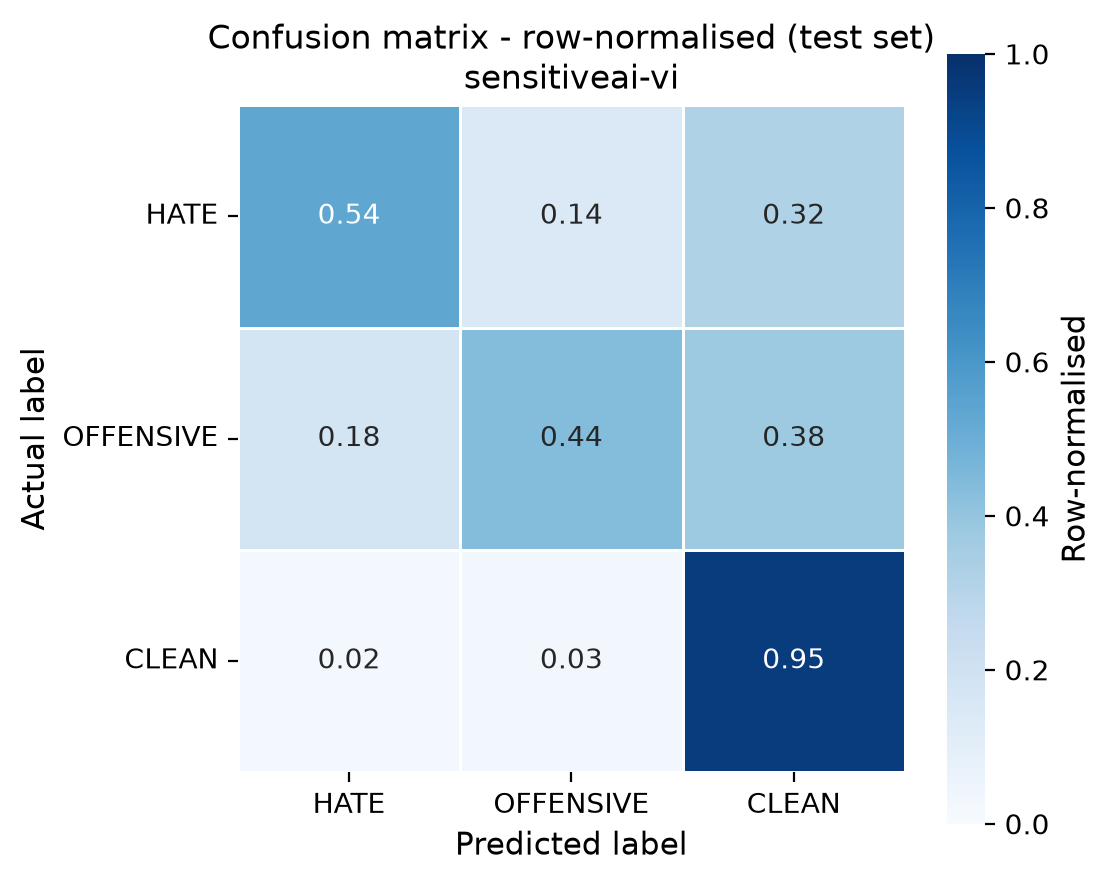
\includegraphics[width=\linewidth]{figures/per_model/M1/confusion_matrix_normalized.png}\caption{Normalised confusion matrix (rows = true, columns = predicted).}\end{minipage}
\end{figure}

\begin{figure}[htbp]
\centering
\begin{minipage}{0.74\textwidth}\centering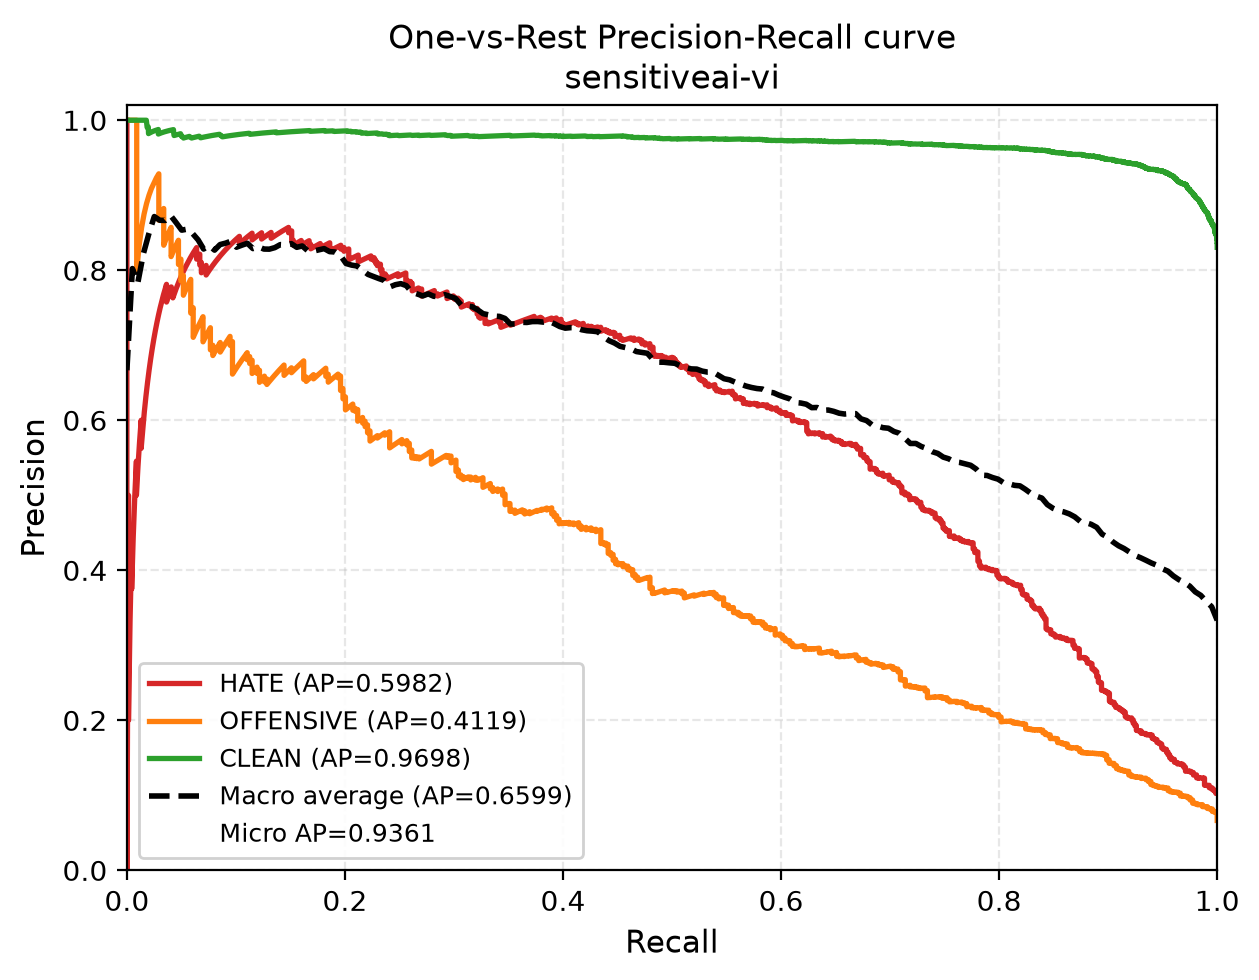
\includegraphics[width=\linewidth]{figures/per_model/M1/pr_curve.png}\caption{Precision--recall curve.}\end{minipage}
\end{figure}

\begin{figure}[htbp]
\centering
\begin{minipage}{0.74\textwidth}\centering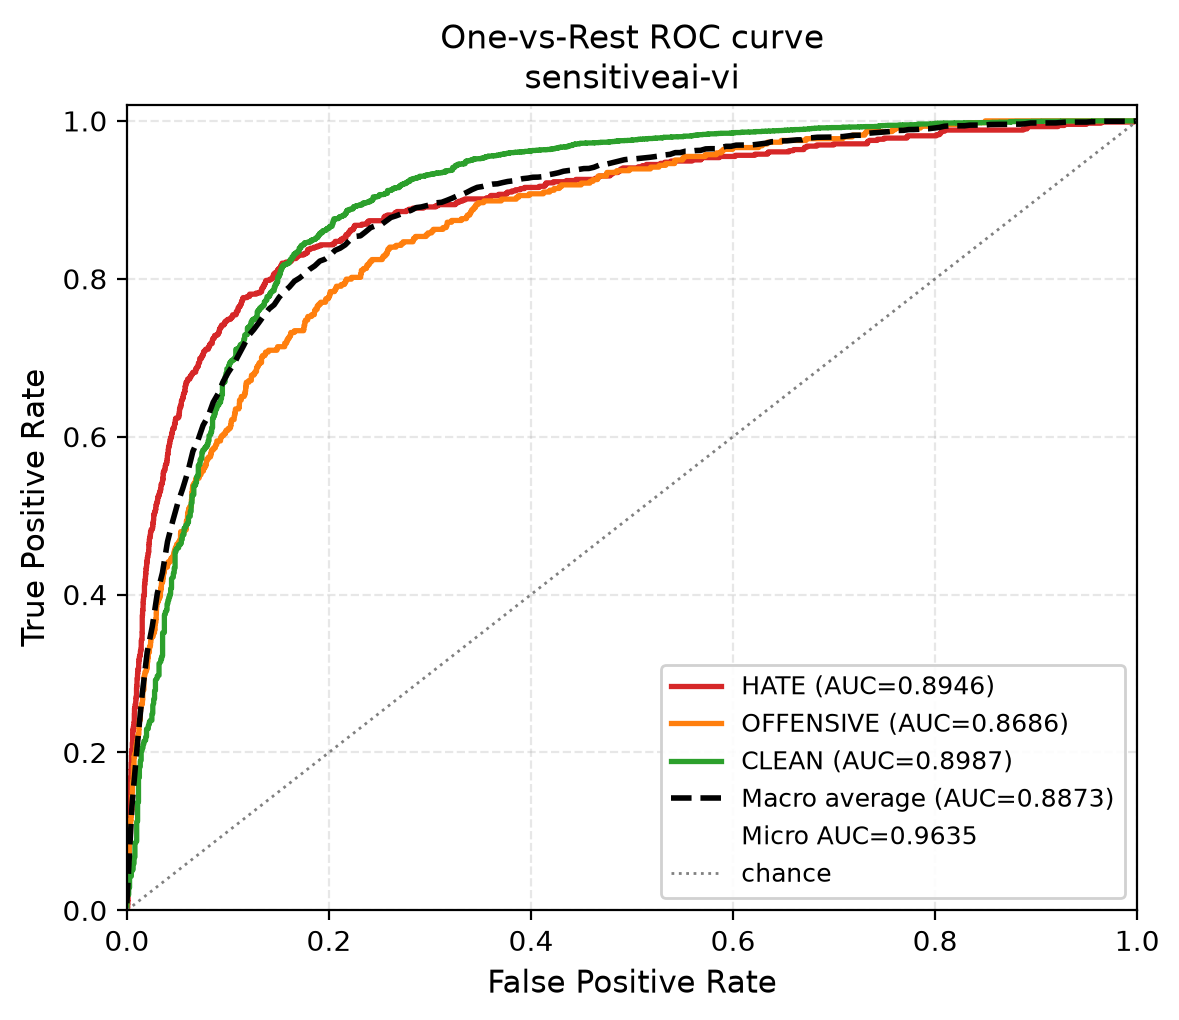
\includegraphics[width=\linewidth]{figures/per_model/M1/roc_curve.png}\caption{ROC curve.}\end{minipage}
\end{figure}

\begin{figure}[htbp]
\centering
\begin{minipage}{0.74\textwidth}\centering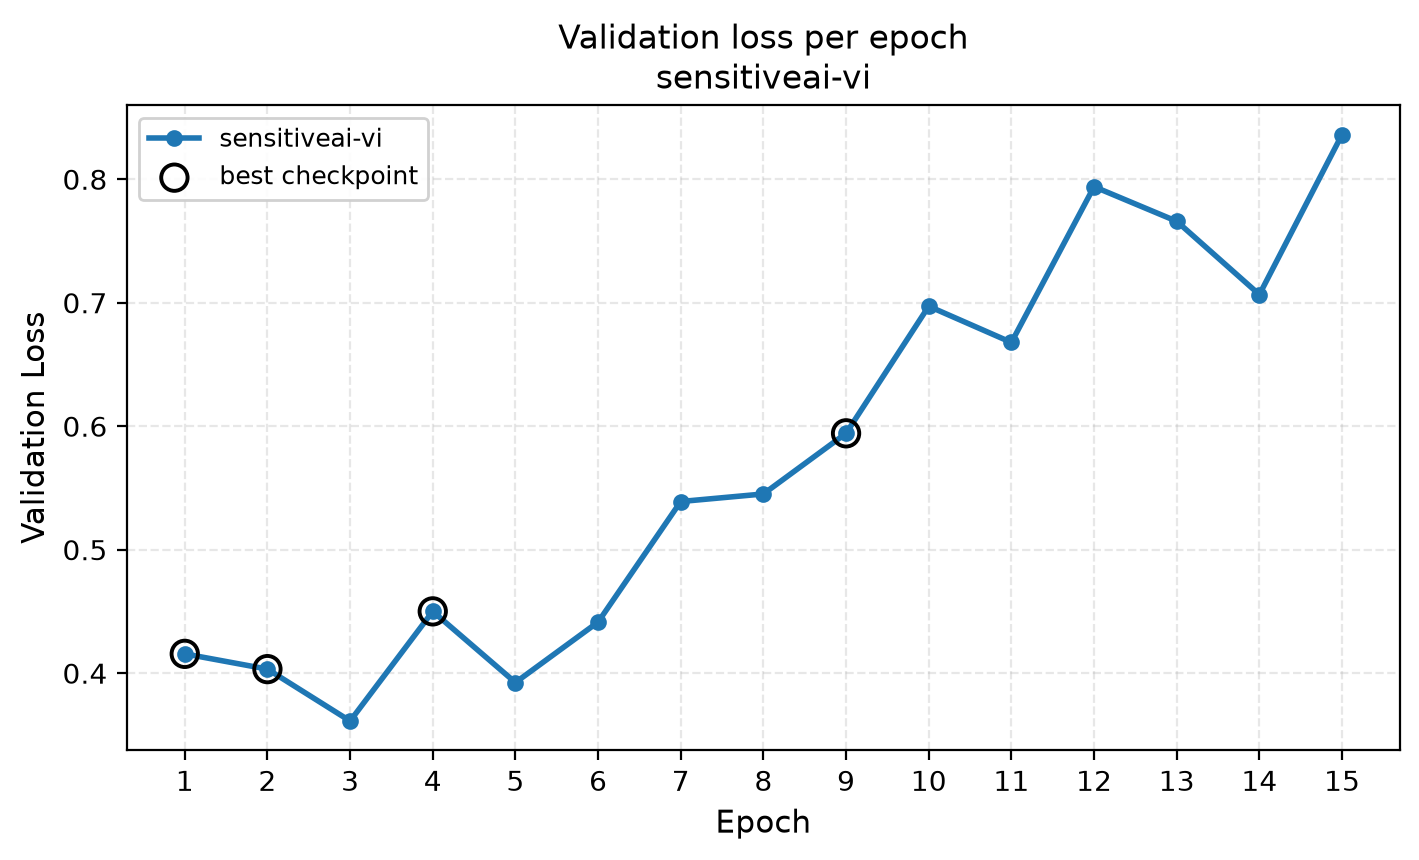
\includegraphics[width=\linewidth]{figures/per_model/M1/val_loss_curve.png}\caption{Validation loss over the training epochs.}\end{minipage}
\end{figure}

\begin{figure}[htbp]
\centering
\begin{minipage}{0.74\textwidth}\centering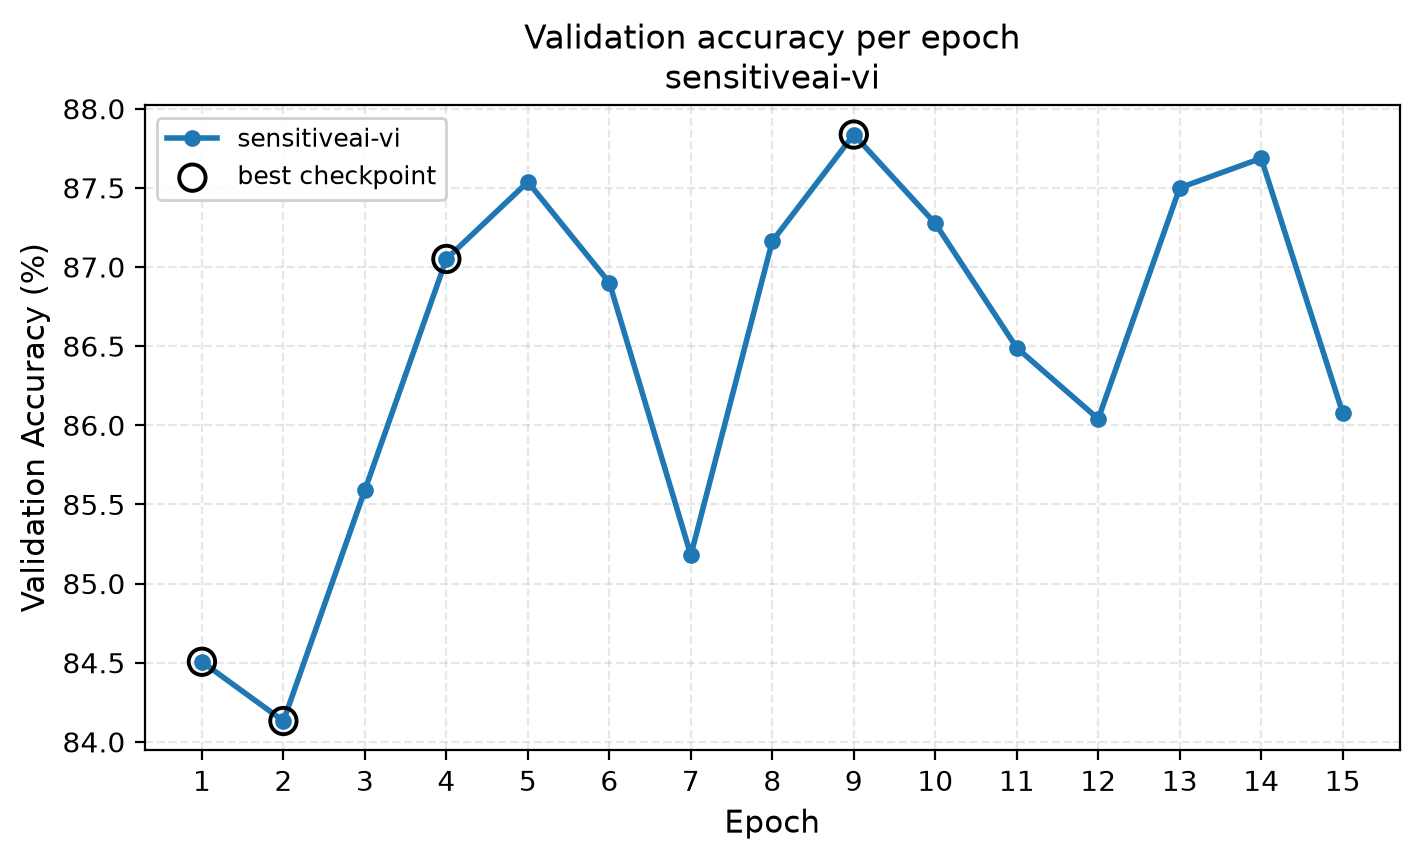
\includegraphics[width=\linewidth]{figures/per_model/M1/val_accuracy_curve.png}\caption{Validation accuracy over the training epochs.}\end{minipage}
\end{figure}


\subsection{\model{M2}}
\label{sec:supp-per-m2}
Baseline plus a \emph{multi-view pooling} head: the first token (\texttt{[CLS]}), masked-mean and masked-max views are concatenated to a 2{,}304-d vector and passed through a LayerNorm $\to$ Linear($2304\to512$) $\to$ GELU $\to$ dropout bottleneck MLP ($512\to3$).  There is no convolutional layer and the optional attention-pooling view is disabled; training is single-stage with plain cross-entropy.

\begin{figure}[htbp]
\centering
\begin{minipage}{0.74\textwidth}\centering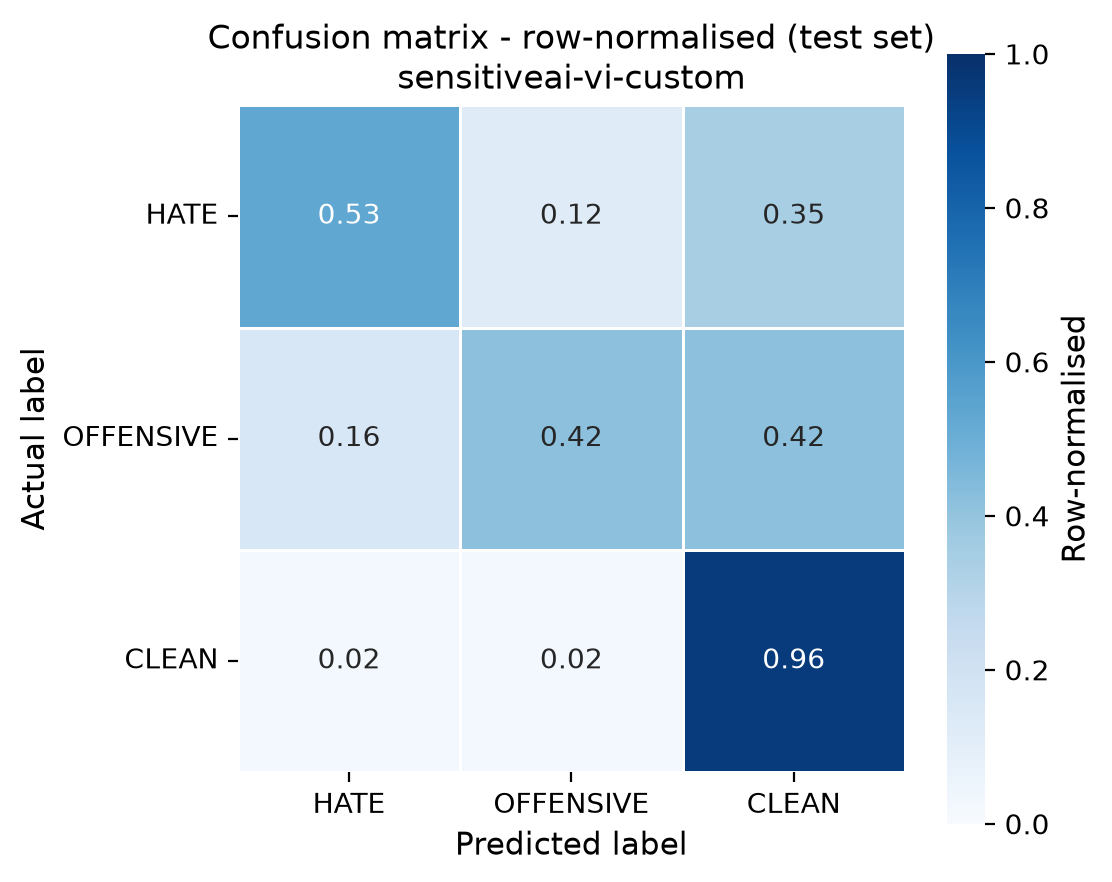
\includegraphics[width=\linewidth]{figures/per_model/M2/confusion_matrix_normalized.png}\caption{Normalised confusion matrix (rows = true, columns = predicted).}\end{minipage}
\end{figure}

\begin{figure}[htbp]
\centering
\begin{minipage}{0.74\textwidth}\centering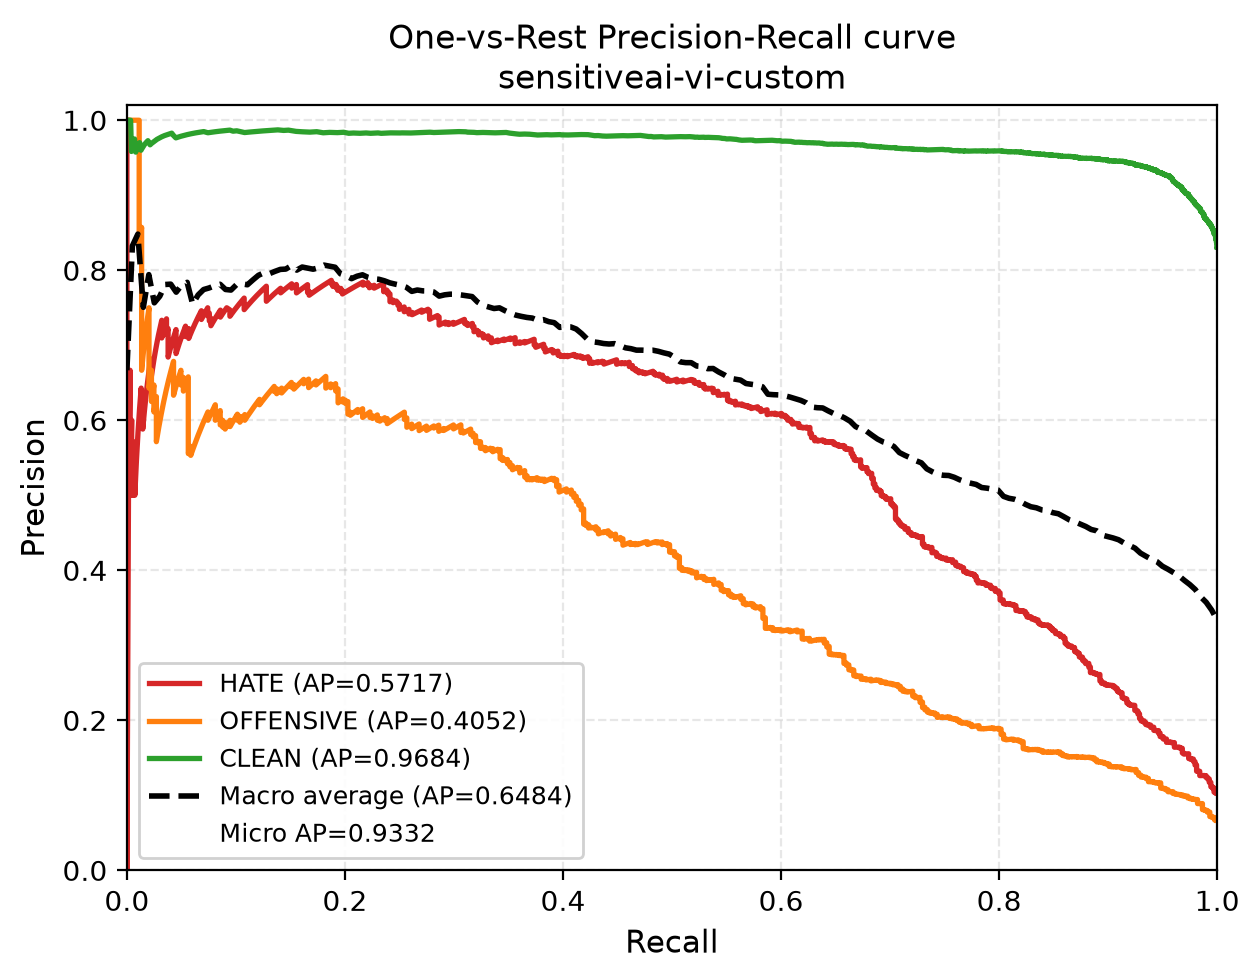
\includegraphics[width=\linewidth]{figures/per_model/M2/pr_curve.png}\caption{Precision--recall curve.}\end{minipage}
\end{figure}

\begin{figure}[htbp]
\centering
\begin{minipage}{0.74\textwidth}\centering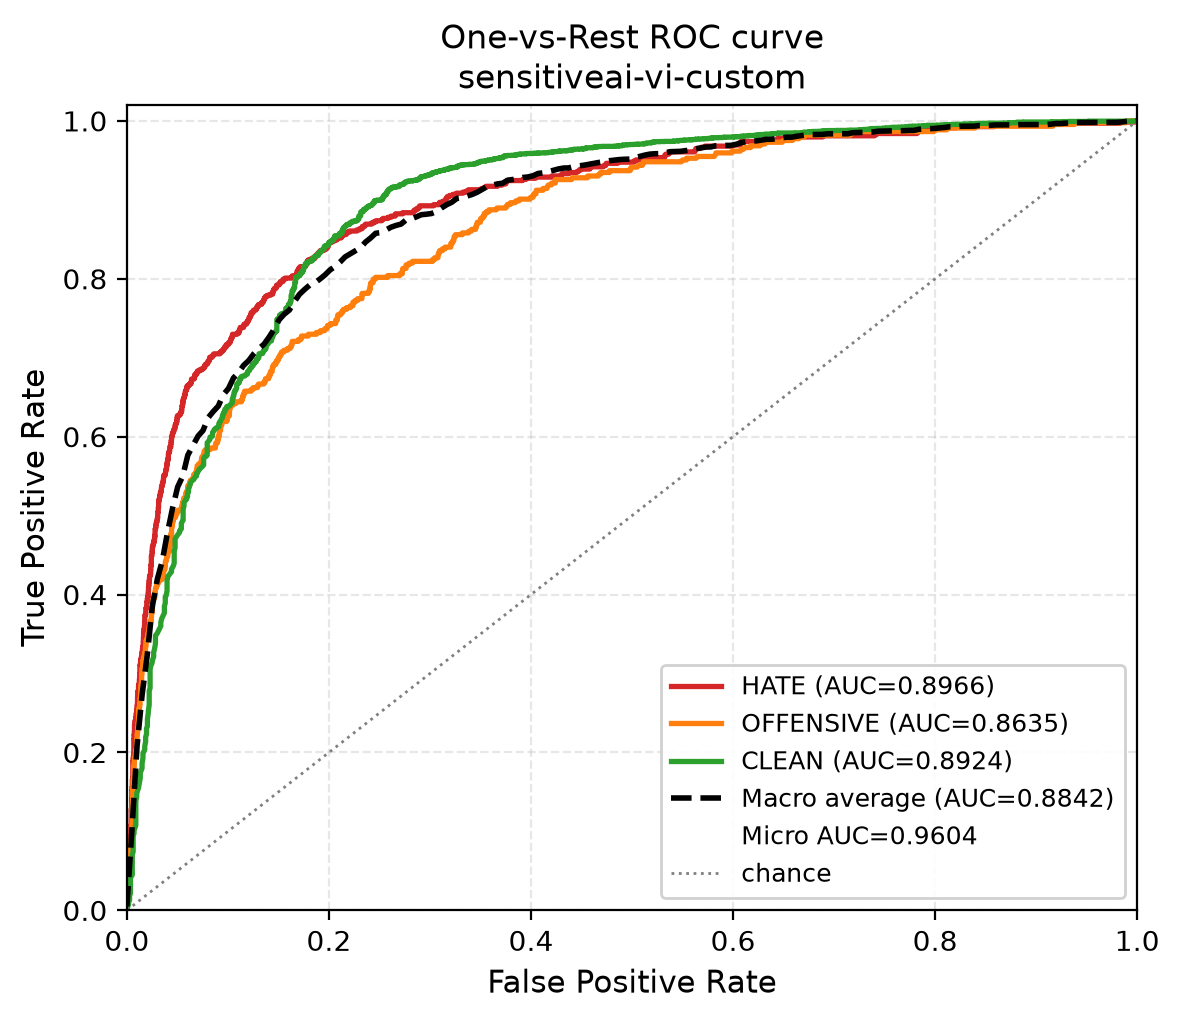
\includegraphics[width=\linewidth]{figures/per_model/M2/roc_curve.png}\caption{ROC curve.}\end{minipage}
\end{figure}

\begin{figure}[htbp]
\centering
\begin{minipage}{0.74\textwidth}\centering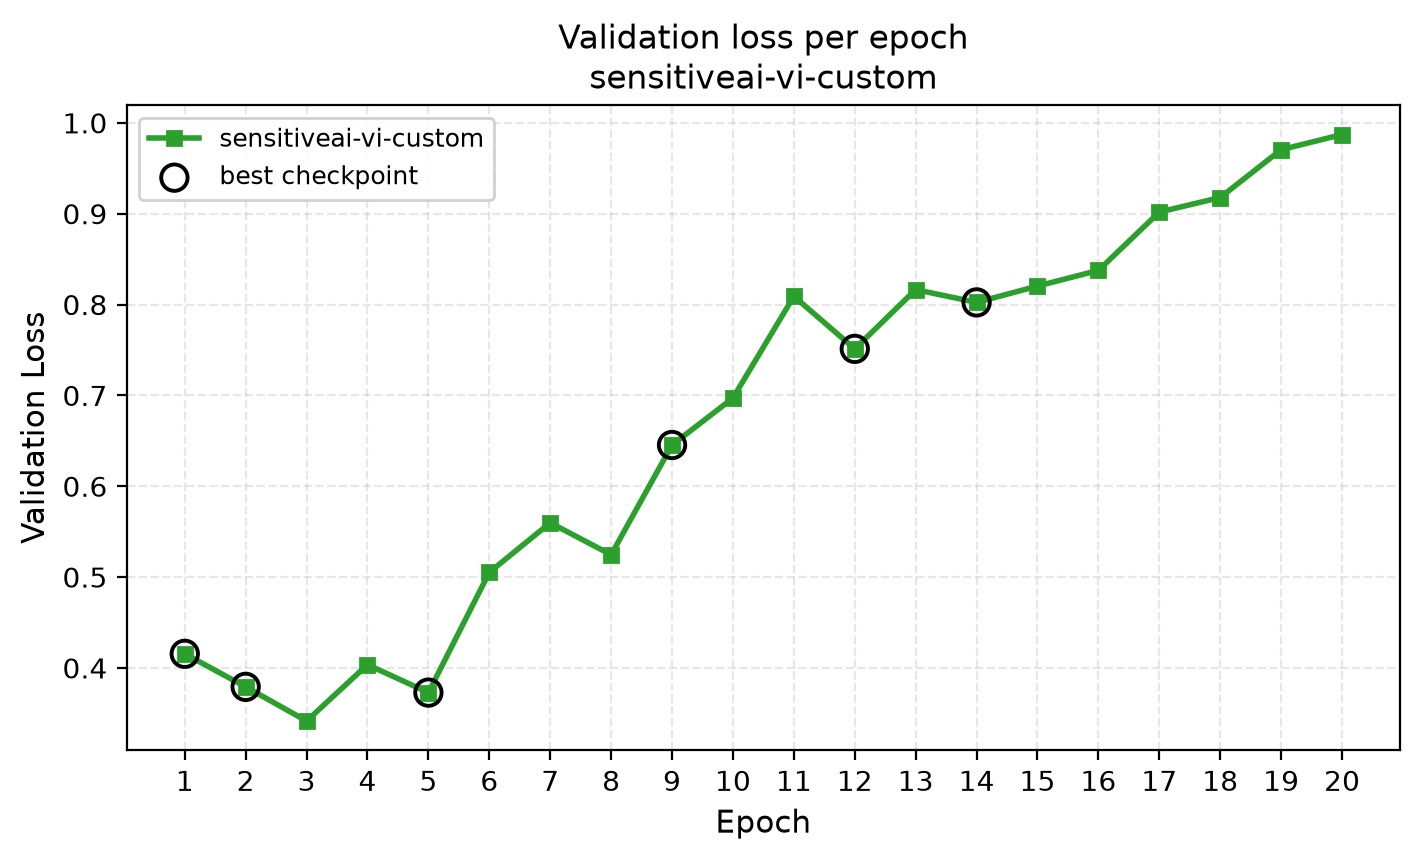
\includegraphics[width=\linewidth]{figures/per_model/M2/val_loss_curve.png}\caption{Validation loss over the training epochs.}\end{minipage}
\end{figure}

\begin{figure}[htbp]
\centering
\begin{minipage}{0.74\textwidth}\centering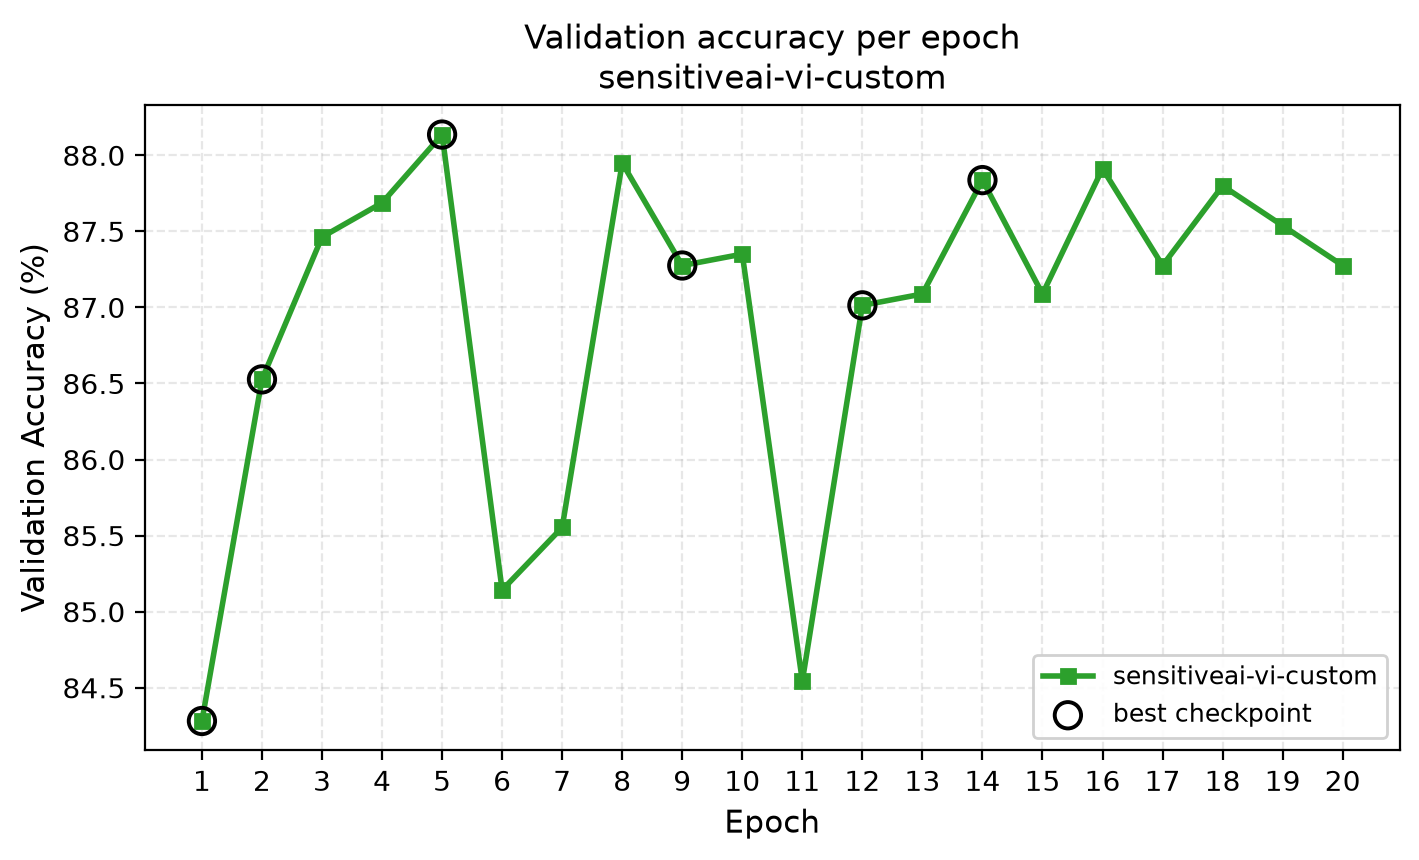
\includegraphics[width=\linewidth]{figures/per_model/M2/val_accuracy_curve.png}\caption{Validation accuracy over the training epochs.}\end{minipage}
\end{figure}


\subsection{\model{M3}}
\label{sec:supp-per-m3}
Multi-view pooling head with discriminative learning rates and a second focal-loss stage; the best macro-F1 of the six ($0.6638$) and the highest MCC.  Its threshold search returned the trivial $0.5$.

\begin{figure}[htbp]
\centering
\begin{minipage}{0.74\textwidth}\centering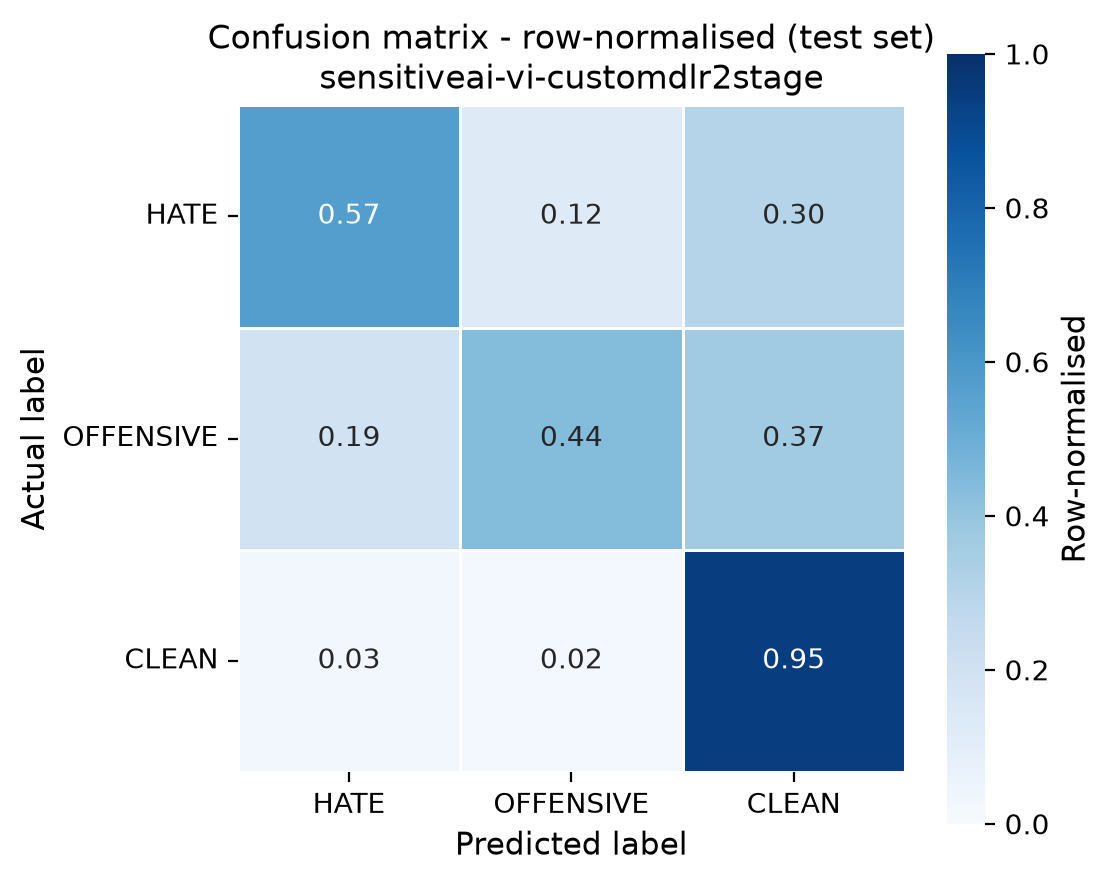
\includegraphics[width=\linewidth]{figures/per_model/M3/confusion_matrix_normalized.png}\caption{Normalised confusion matrix (rows = true, columns = predicted).}\end{minipage}
\end{figure}

\begin{figure}[htbp]
\centering
\begin{minipage}{0.74\textwidth}\centering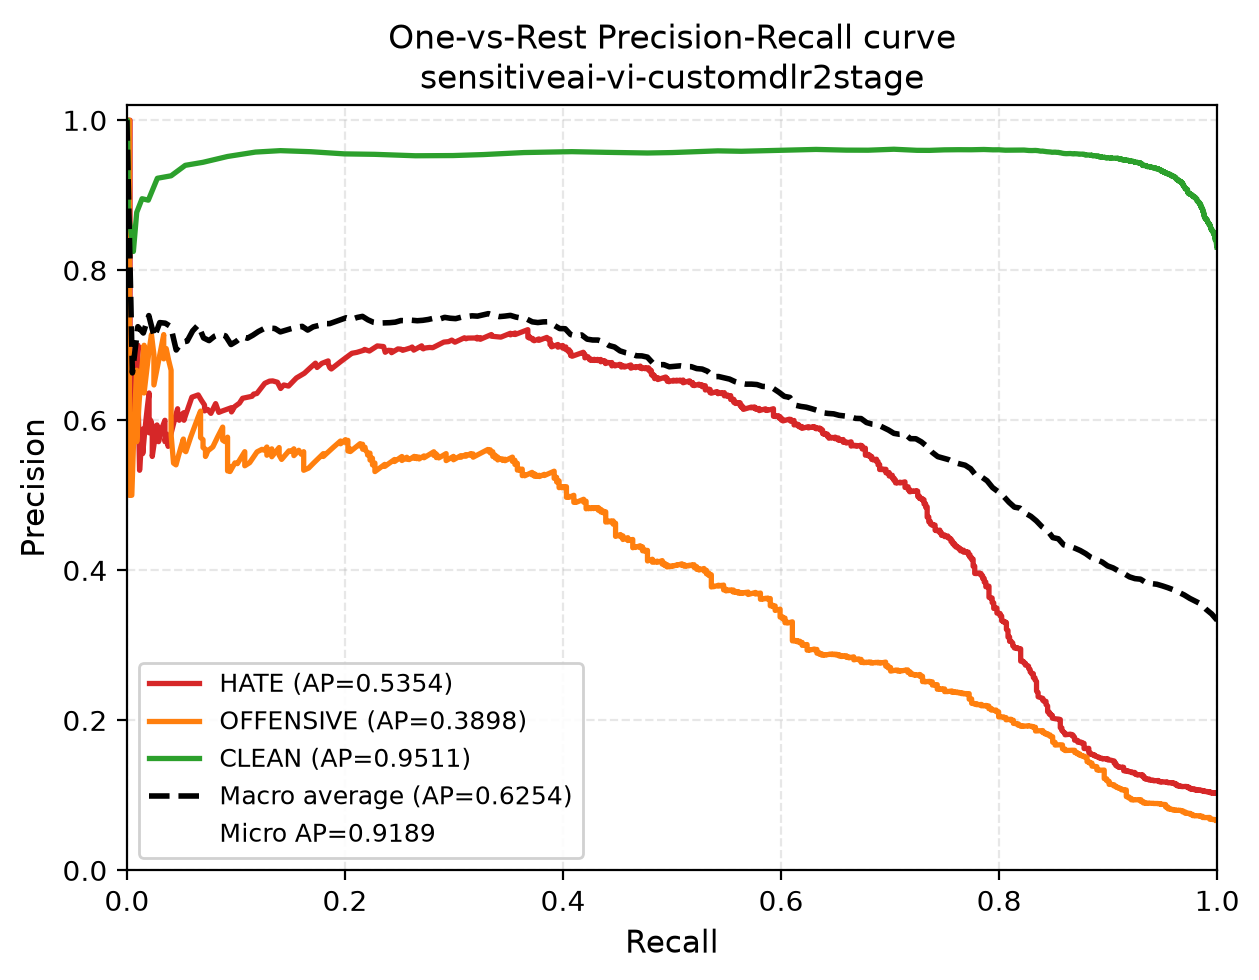
\includegraphics[width=\linewidth]{figures/per_model/M3/pr_curve.png}\caption{Precision--recall curve.}\end{minipage}
\end{figure}

\begin{figure}[htbp]
\centering
\begin{minipage}{0.74\textwidth}\centering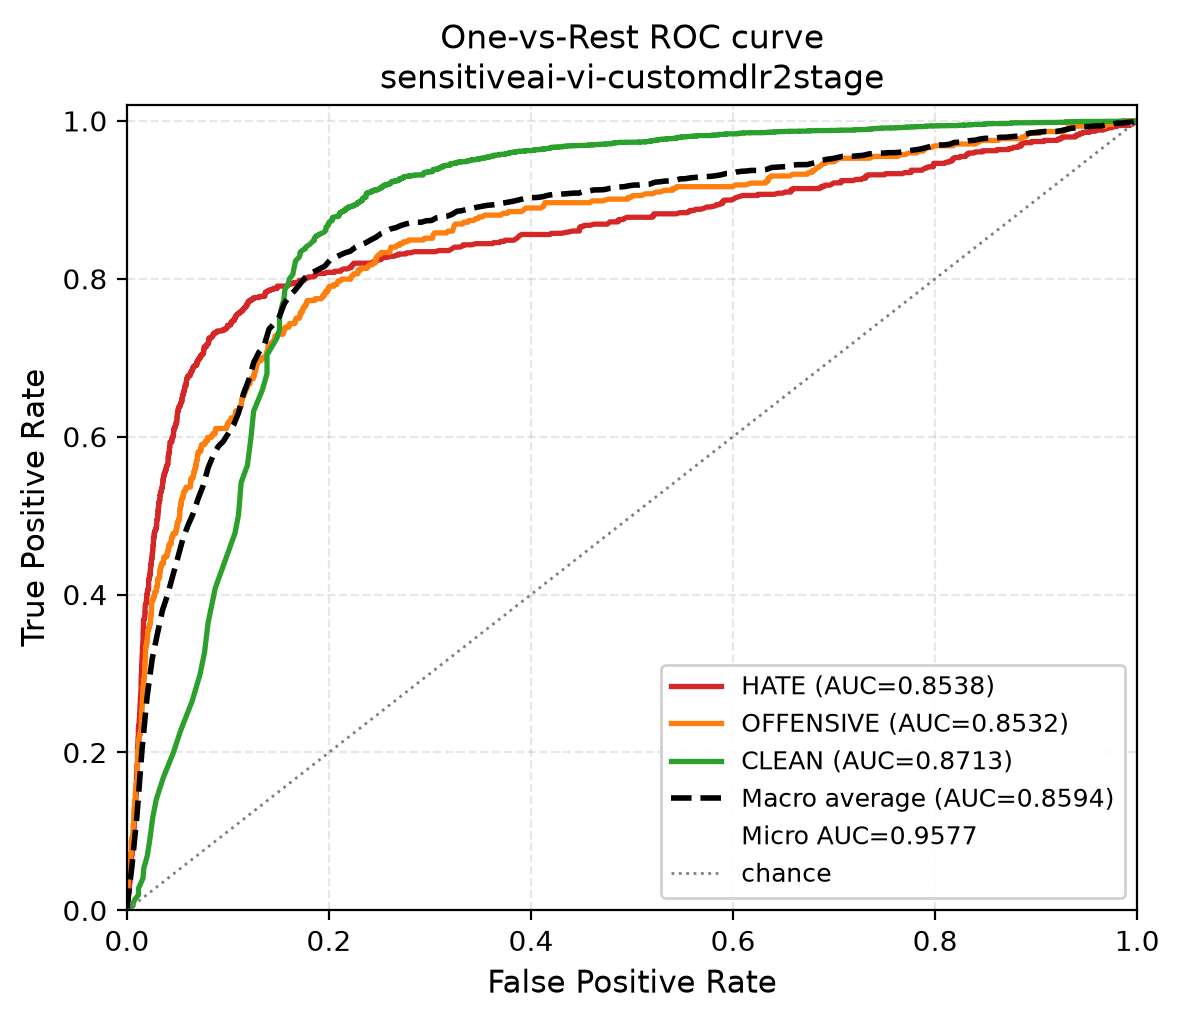
\includegraphics[width=\linewidth]{figures/per_model/M3/roc_curve.png}\caption{ROC curve.}\end{minipage}
\end{figure}

\begin{figure}[htbp]
\centering
\begin{minipage}{0.74\textwidth}\centering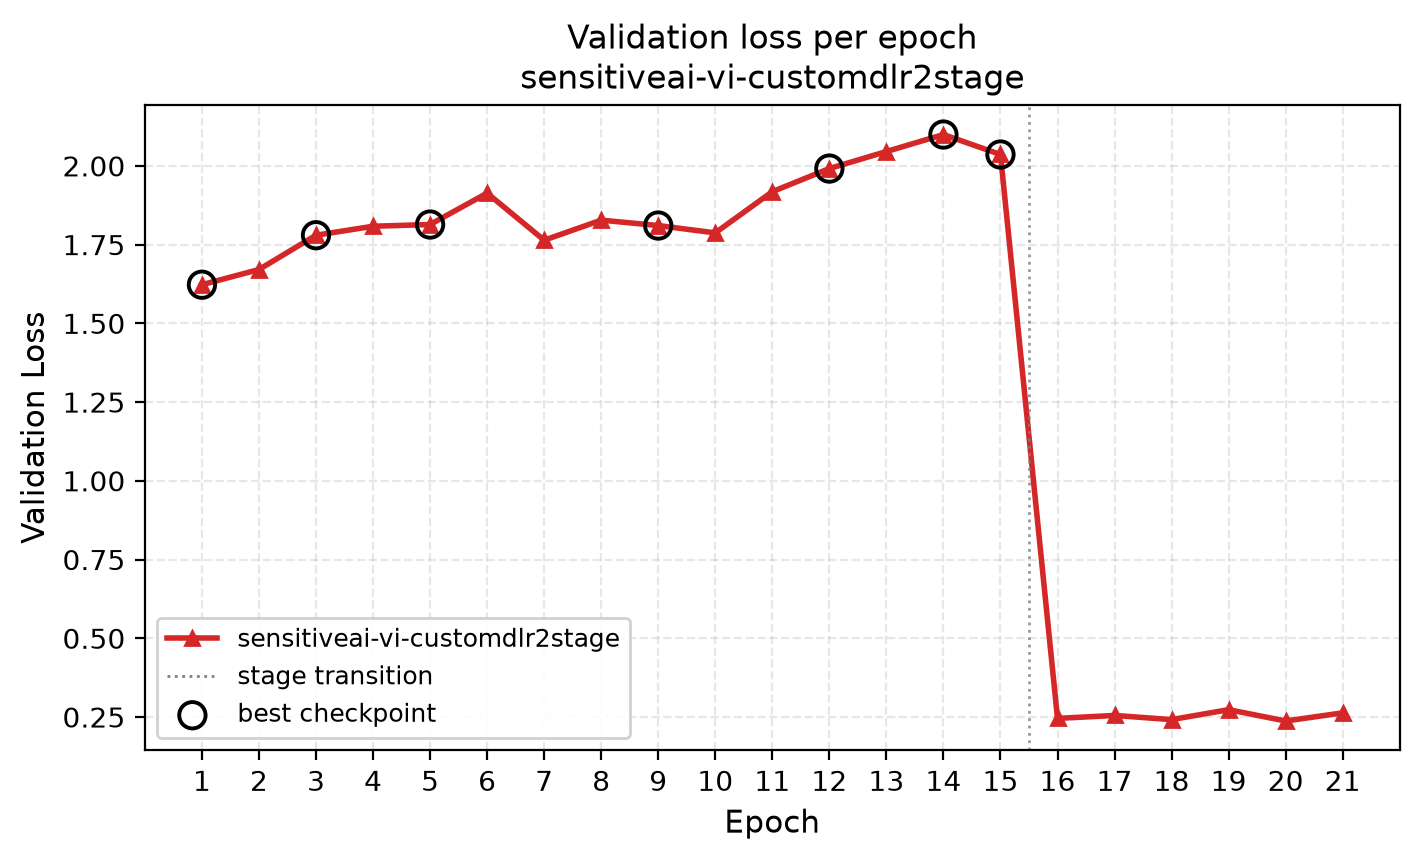
\includegraphics[width=\linewidth]{figures/per_model/M3/val_loss_curve.png}\caption{Validation loss over the training epochs.}\end{minipage}
\end{figure}

\begin{figure}[htbp]
\centering
\begin{minipage}{0.74\textwidth}\centering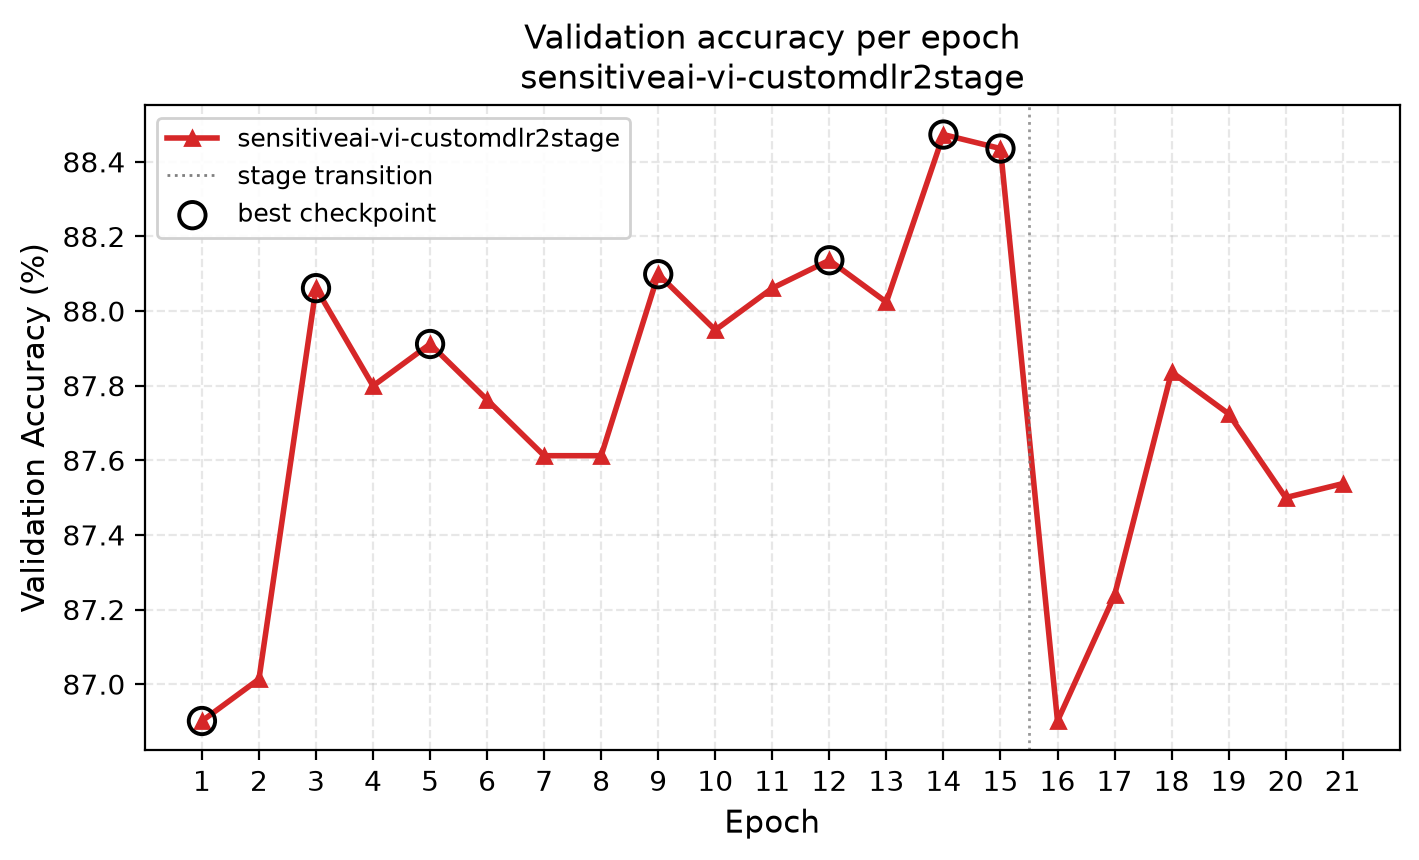
\includegraphics[width=\linewidth]{figures/per_model/M3/val_accuracy_curve.png}\caption{Validation accuracy over the training epochs.}\end{minipage}
\end{figure}


\subsection{\model{M4}}
\label{sec:supp-per-m4}
Multi-view head trained as a three-stage curriculum, initialised from \model{M3}'s checkpoint.  Stage~1 (concept loss, OFFENSIVE) was allocated 10 epochs but early stopping truncated it after 7; stage~2 (concept loss, HATE) ran 6\,(absolute epochs $8$--$13$) and stage~3 (cross-entropy, class weights $3{:}2{:}1$) ran 6\,(absolute epochs $14$--$19$), for $19$ of $30$ planned epochs.  The run's best \emph{validation} macro-F1 ($0.6942$) occurred at absolute epoch~1 and was never beaten, so the later stages were not selected; its searched thresholds ($0.01/0.5/0.64$) raised validation macro-F1 but did not transfer to test.

\begin{figure}[htbp]
\centering
\begin{minipage}{0.74\textwidth}\centering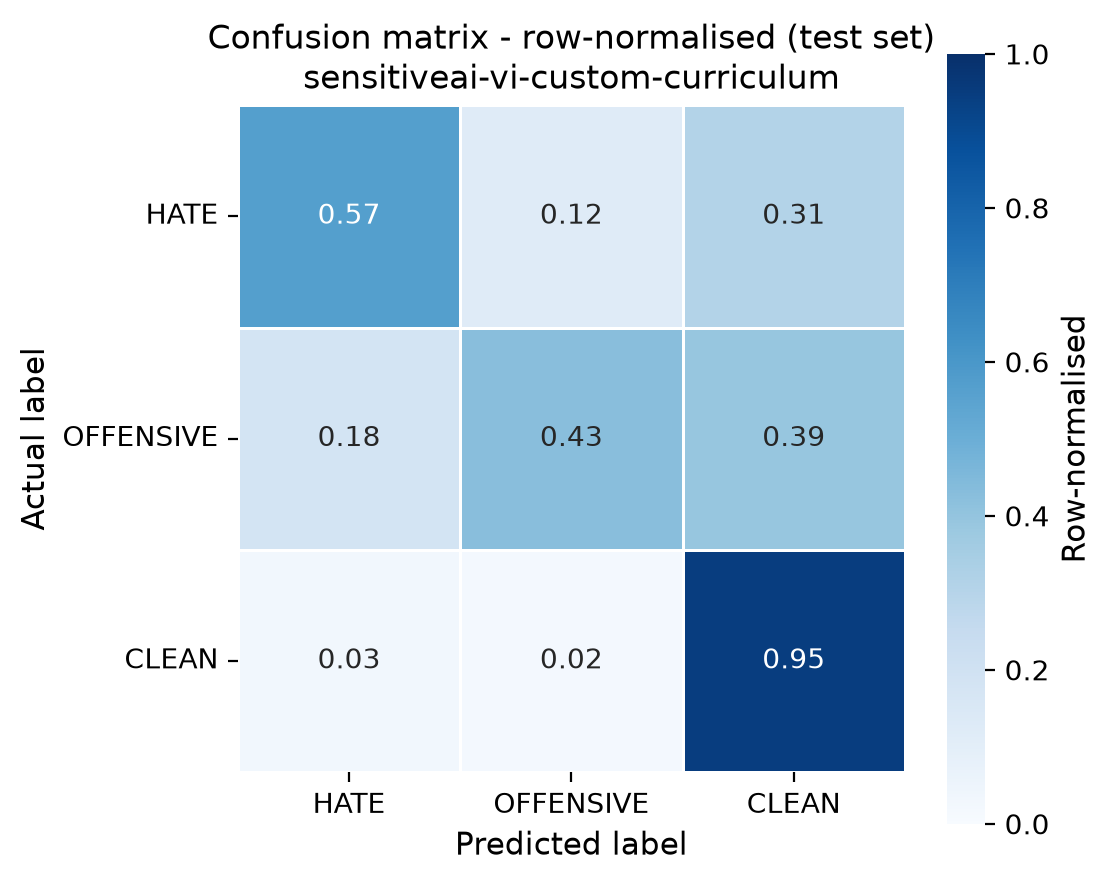
\includegraphics[width=\linewidth]{figures/per_model/M4/confusion_matrix_normalized.png}\caption{Normalised confusion matrix (rows = true, columns = predicted).}\end{minipage}
\end{figure}

\begin{figure}[htbp]
\centering
\begin{minipage}{0.74\textwidth}\centering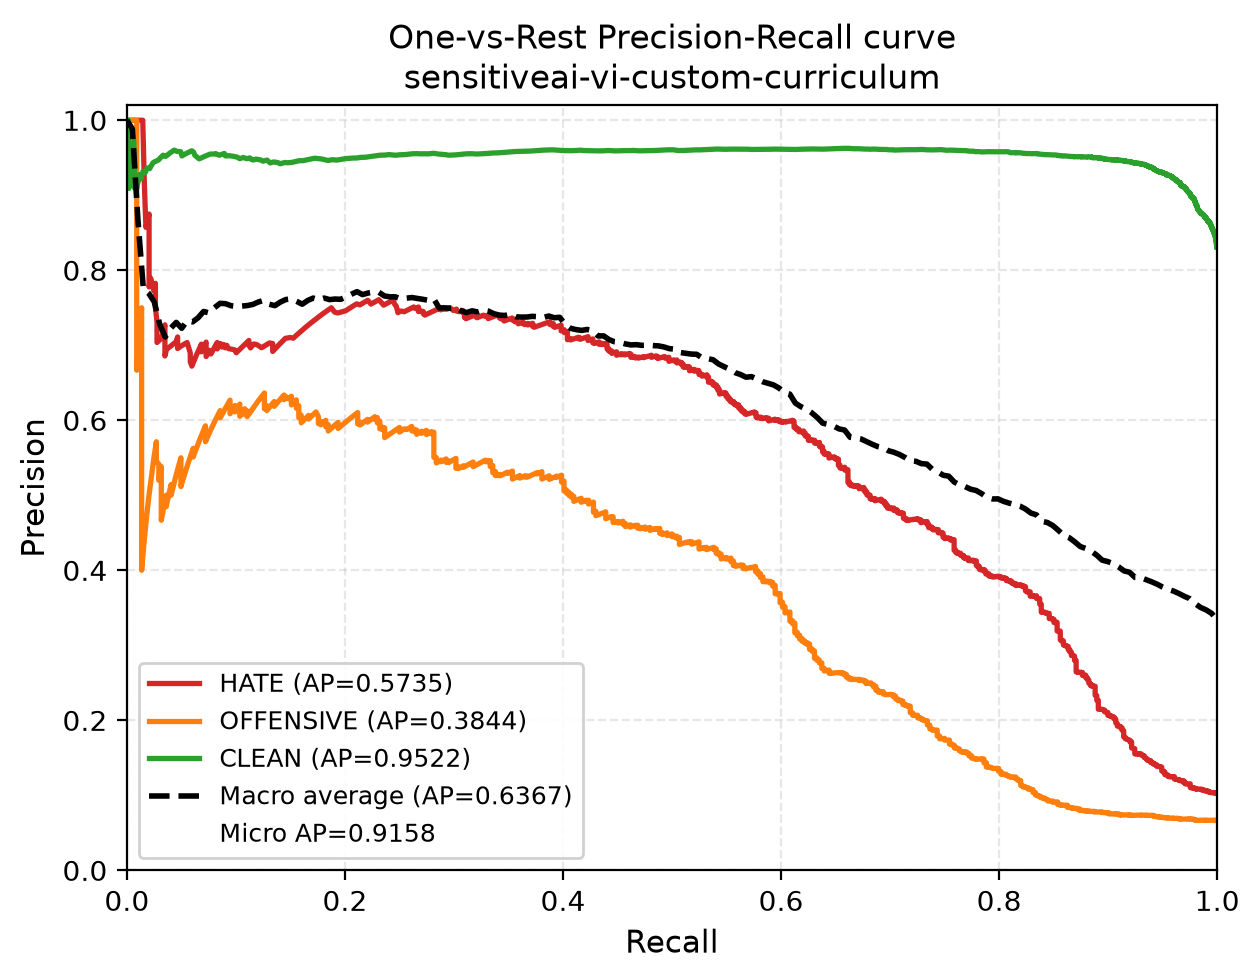
\includegraphics[width=\linewidth]{figures/per_model/M4/pr_curve.png}\caption{Precision--recall curve.}\end{minipage}
\end{figure}

\begin{figure}[htbp]
\centering
\begin{minipage}{0.74\textwidth}\centering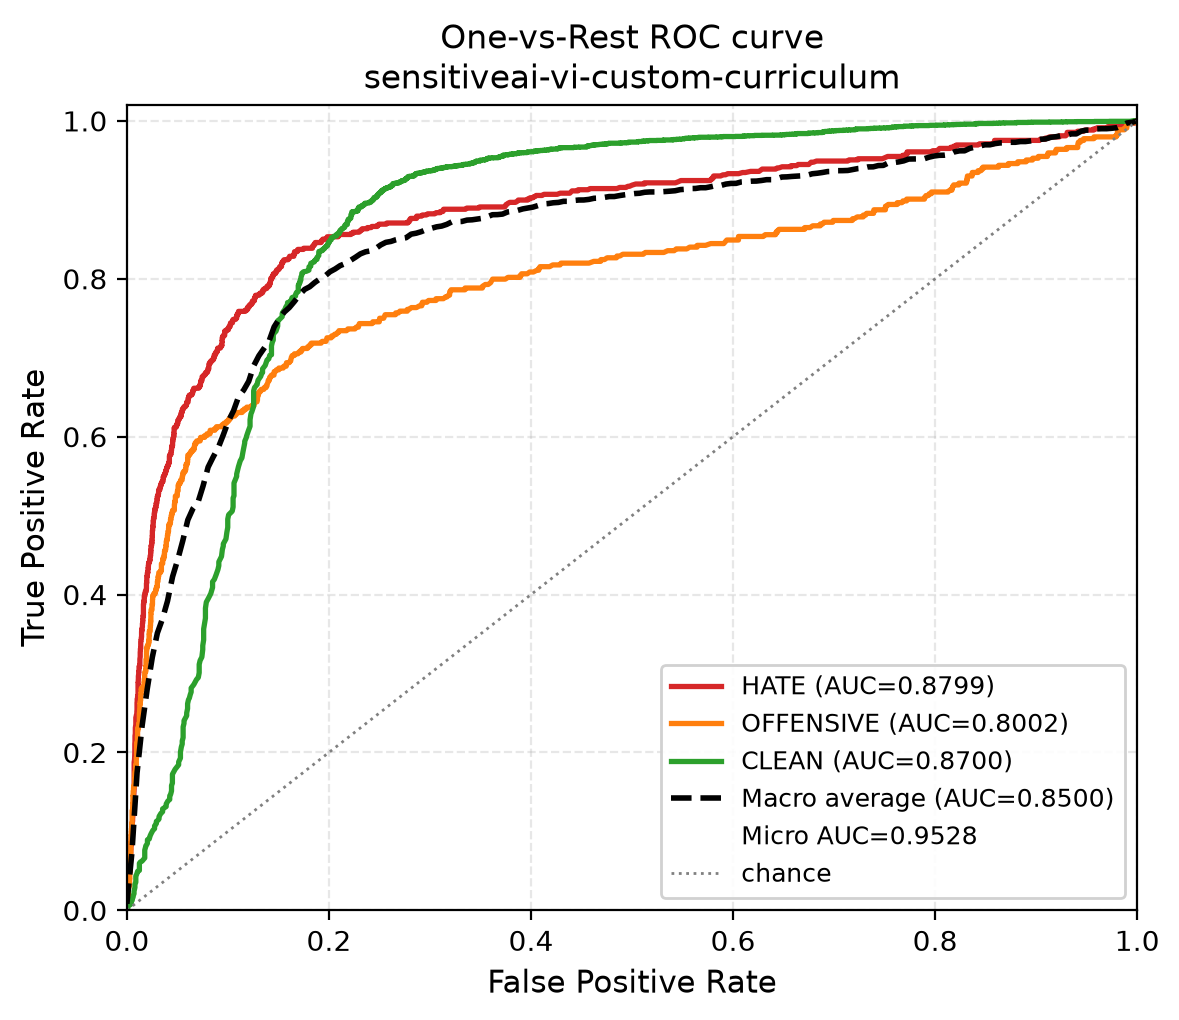
\includegraphics[width=\linewidth]{figures/per_model/M4/roc_curve.png}\caption{ROC curve.}\end{minipage}
\end{figure}

\begin{figure}[htbp]
\centering
\begin{minipage}{0.74\textwidth}\centering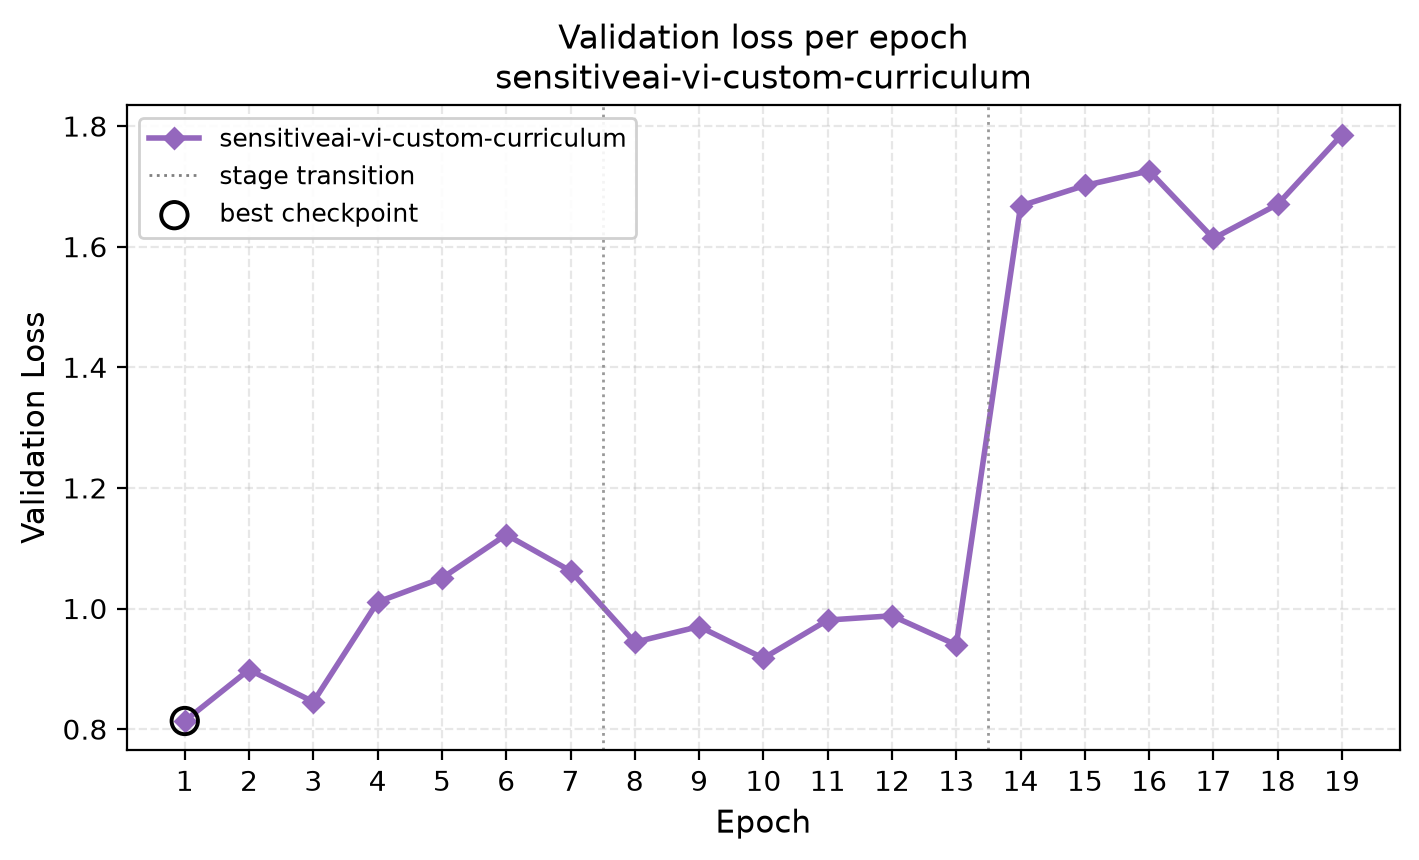
\includegraphics[width=\linewidth]{figures/per_model/M4/val_loss_curve.png}\caption{Validation loss over the training epochs.}\end{minipage}
\end{figure}

\begin{figure}[htbp]
\centering
\begin{minipage}{0.74\textwidth}\centering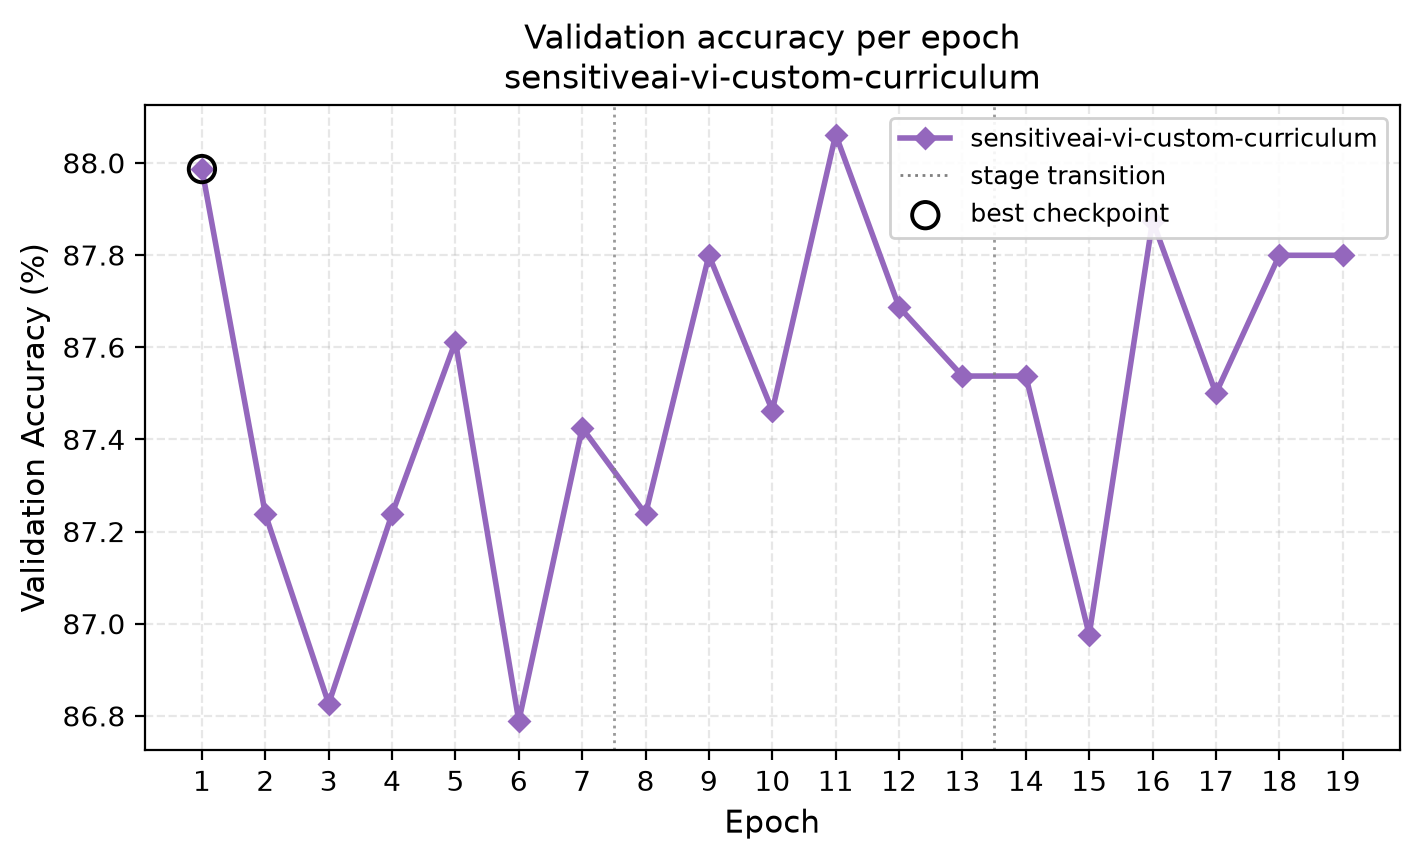
\includegraphics[width=\linewidth]{figures/per_model/M4/val_accuracy_curve.png}\caption{Validation accuracy over the training epochs.}\end{minipage}
\end{figure}


\subsection{\model{M5}}
\label{sec:supp-per-m5}
Continuation of \model{M3}'s stage-1 recipe (DLR plus class-weighted cross-entropy) for a further 15 epochs, reaching the full budget because the early-stopping patience equals the budget and could not trigger earlier.  It has the \emph{highest} test accuracy ($0.878$) but the \emph{lowest} macro-F1 ($0.654$)---the accuracy/macro-F1 trap in one system.

\begin{figure}[htbp]
\centering
\begin{minipage}{0.74\textwidth}\centering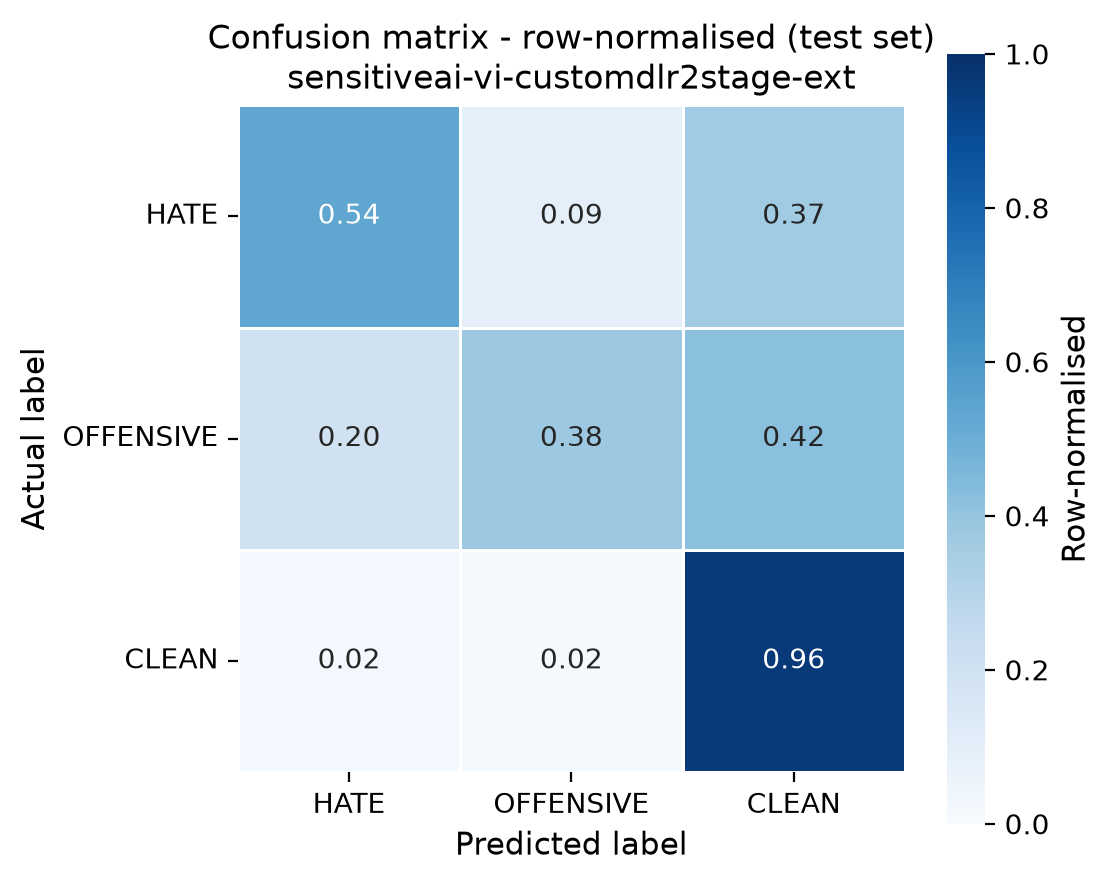
\includegraphics[width=\linewidth]{figures/per_model/M5/confusion_matrix_normalized.png}\caption{Normalised confusion matrix (rows = true, columns = predicted).}\end{minipage}
\end{figure}

\begin{figure}[htbp]
\centering
\begin{minipage}{0.74\textwidth}\centering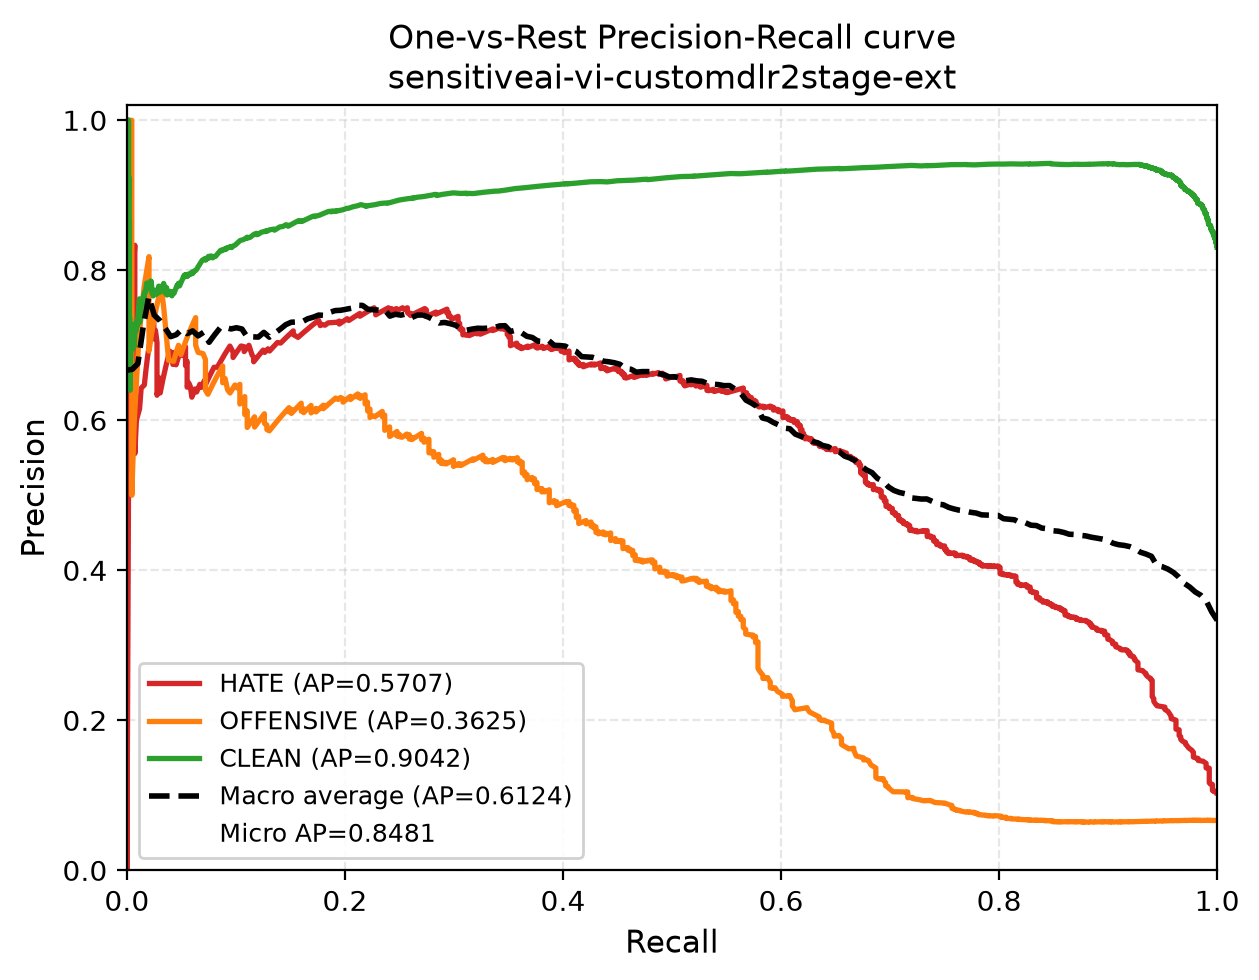
\includegraphics[width=\linewidth]{figures/per_model/M5/pr_curve.png}\caption{Precision--recall curve.}\end{minipage}
\end{figure}

\begin{figure}[htbp]
\centering
\begin{minipage}{0.74\textwidth}\centering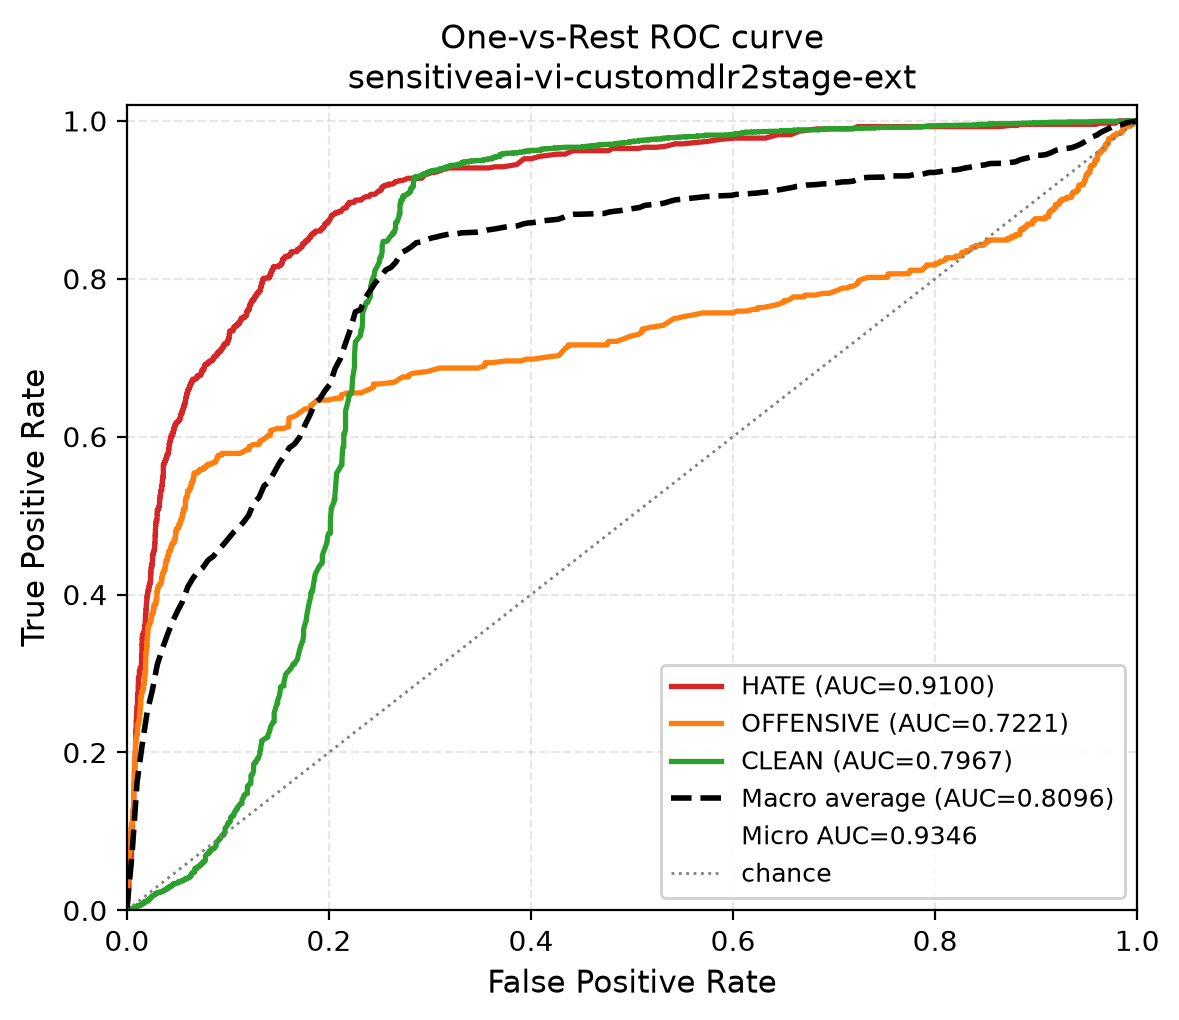
\includegraphics[width=\linewidth]{figures/per_model/M5/roc_curve.png}\caption{ROC curve.}\end{minipage}
\end{figure}

\begin{figure}[htbp]
\centering
\begin{minipage}{0.74\textwidth}\centering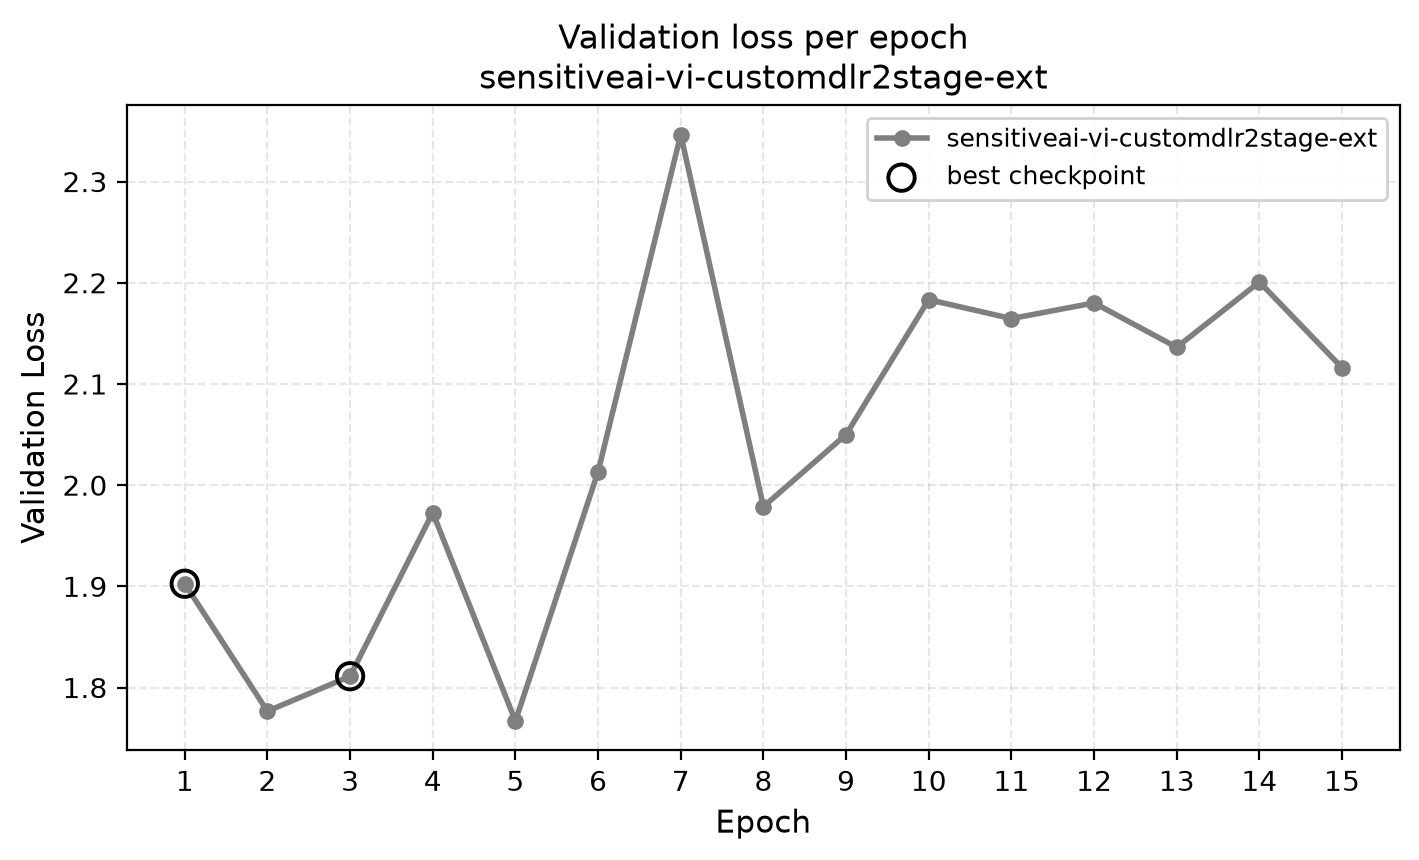
\includegraphics[width=\linewidth]{figures/per_model/M5/val_loss_curve.png}\caption{Validation loss over the training epochs.}\end{minipage}
\end{figure}

\begin{figure}[htbp]
\centering
\begin{minipage}{0.74\textwidth}\centering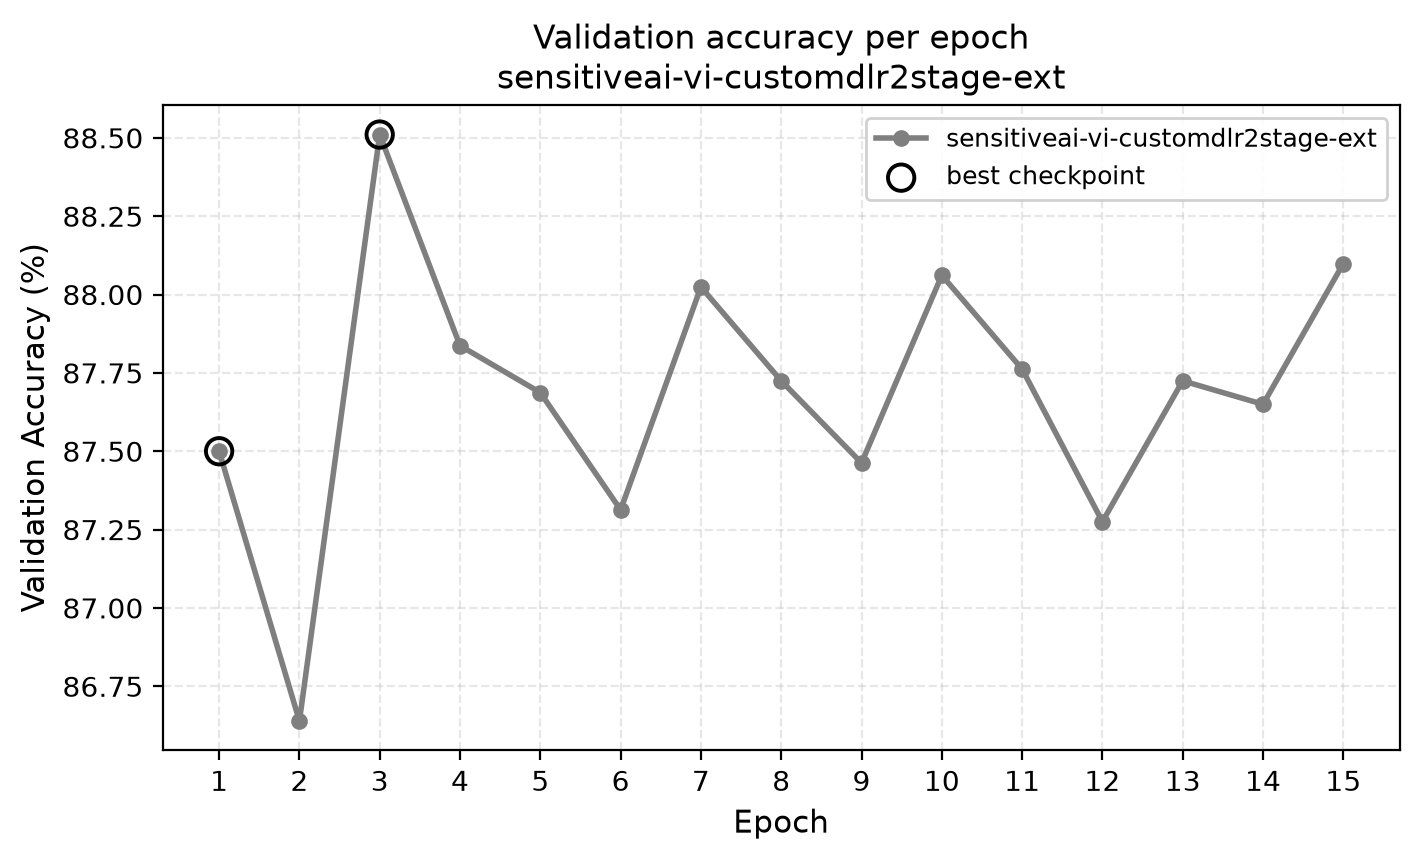
\includegraphics[width=\linewidth]{figures/per_model/M5/val_accuracy_curve.png}\caption{Validation accuracy over the training epochs.}\end{minipage}
\end{figure}


\subsection{\model{M6}}
\label{sec:supp-per-m6}
A focal-only second stage on the baseline head (class-weighted focal loss, no multi-view head).  It has the best HATE recall ($0.647$), the best HATE F1 ($0.609$) and the best macro ROC-AUC ($0.893$), but the lowest CLEAN recall ($0.922$) and the lowest accuracy ($0.863$).

\begin{figure}[htbp]
\centering
\begin{minipage}{0.74\textwidth}\centering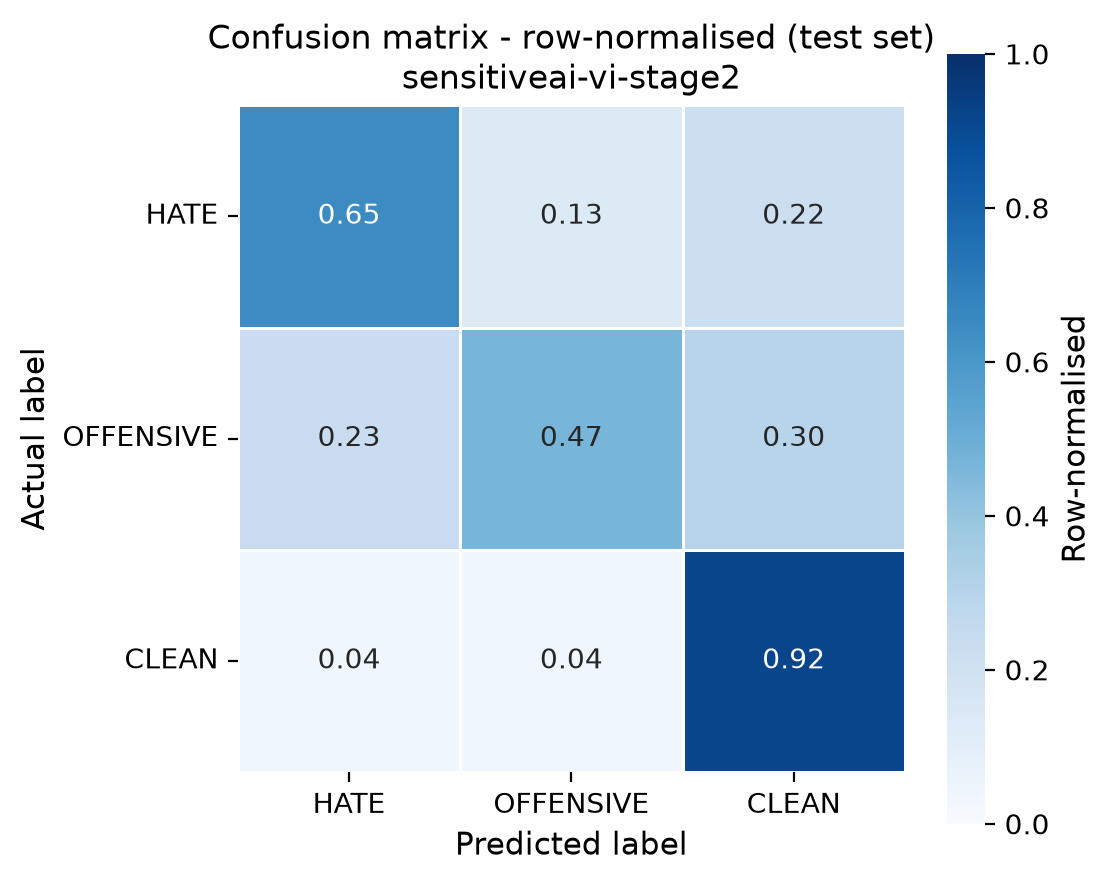
\includegraphics[width=\linewidth]{figures/per_model/M6/confusion_matrix_normalized.png}\caption{Normalised confusion matrix (rows = true, columns = predicted).}\end{minipage}
\end{figure}

\begin{figure}[htbp]
\centering
\begin{minipage}{0.74\textwidth}\centering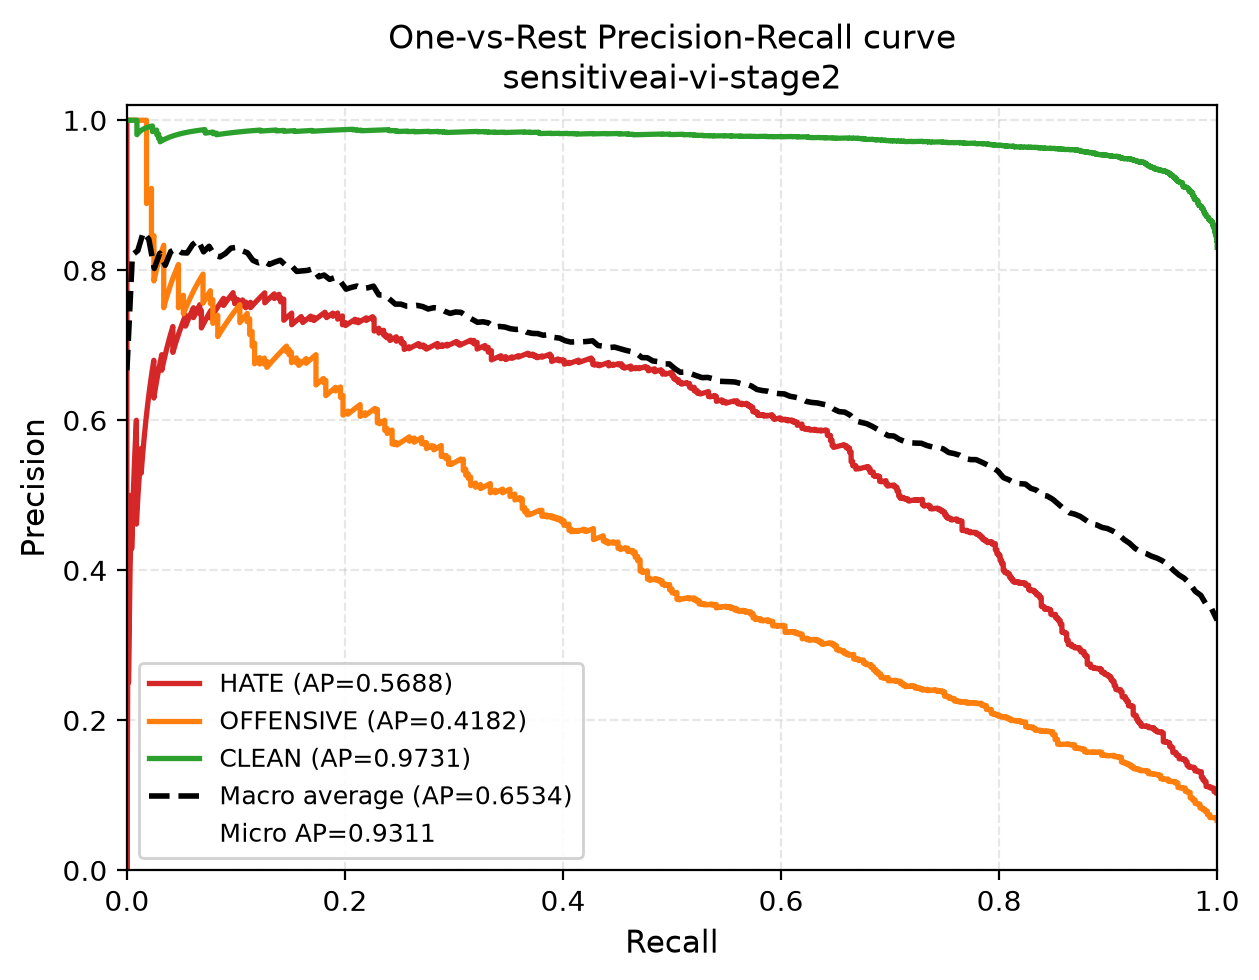
\includegraphics[width=\linewidth]{figures/per_model/M6/pr_curve.png}\caption{Precision--recall curve.}\end{minipage}
\end{figure}

\begin{figure}[htbp]
\centering
\begin{minipage}{0.74\textwidth}\centering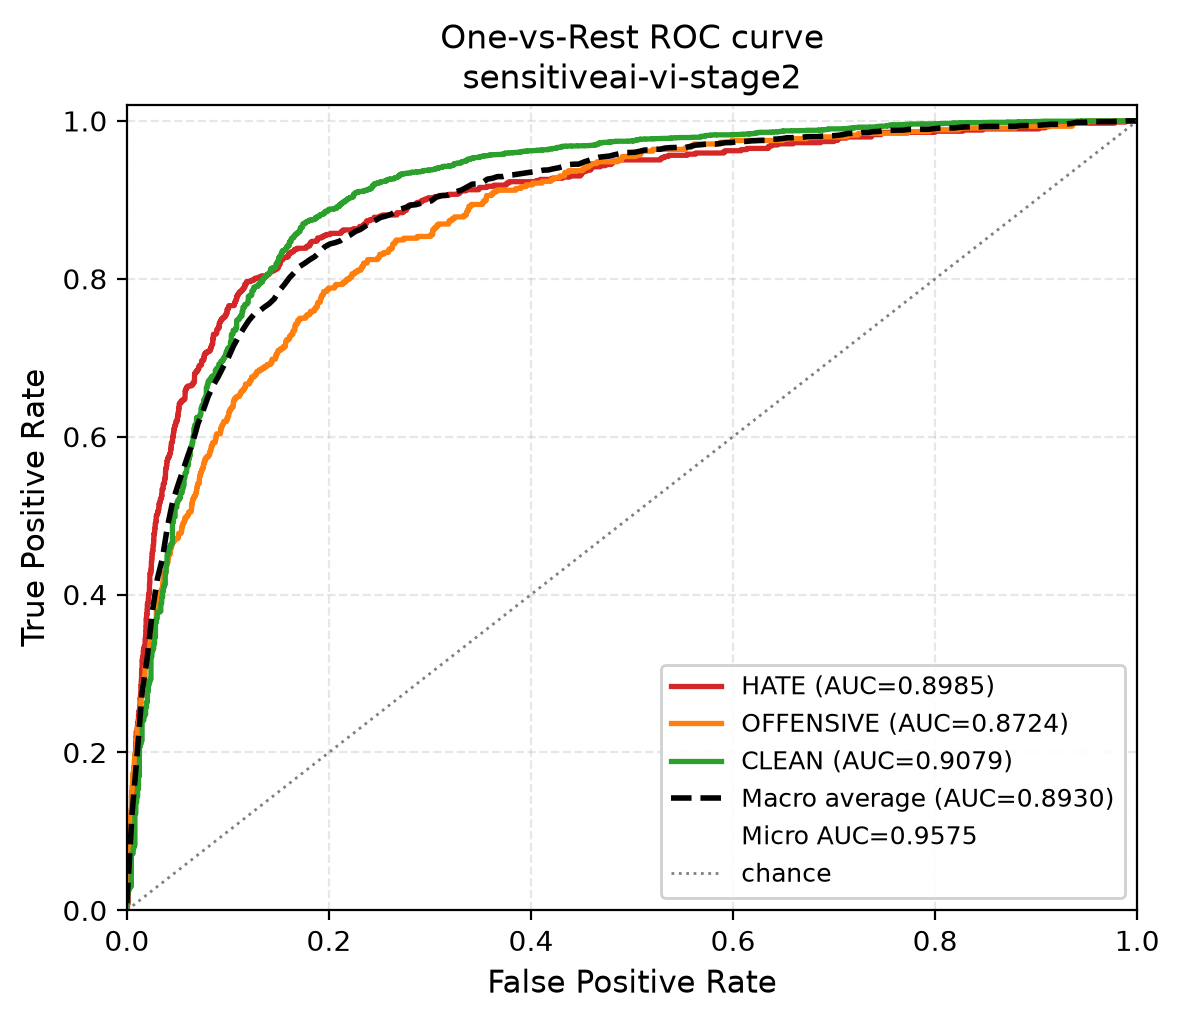
\includegraphics[width=\linewidth]{figures/per_model/M6/roc_curve.png}\caption{ROC curve.}\end{minipage}
\end{figure}

\begin{figure}[htbp]
\centering
\begin{minipage}{0.74\textwidth}\centering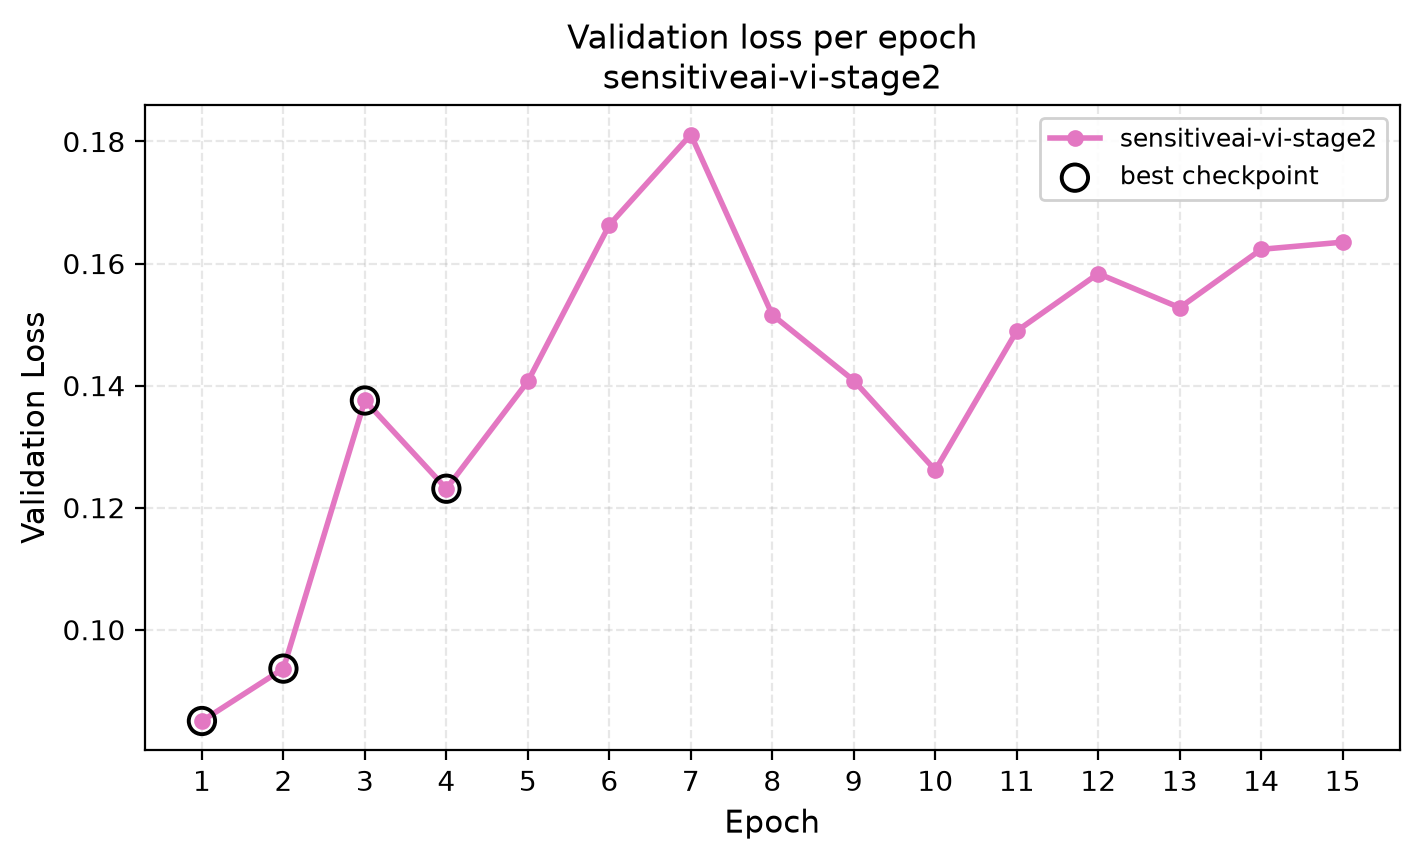
\includegraphics[width=\linewidth]{figures/per_model/M6/val_loss_curve.png}\caption{Validation loss over the training epochs.}\end{minipage}
\end{figure}

\begin{figure}[htbp]
\centering
\begin{minipage}{0.74\textwidth}\centering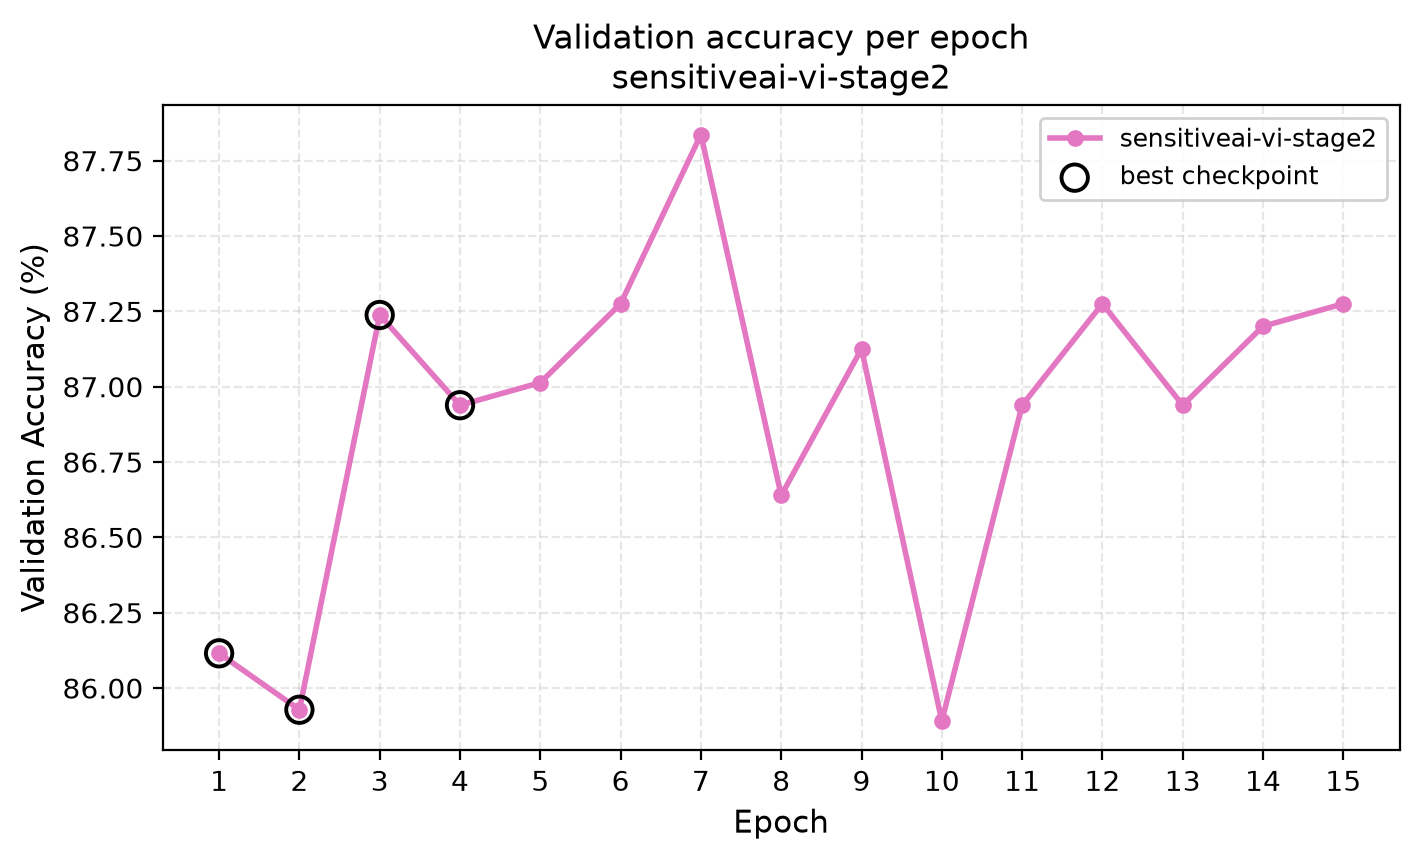
\includegraphics[width=\linewidth]{figures/per_model/M6/val_accuracy_curve.png}\caption{Validation accuracy over the training epochs.}\end{minipage}
\end{figure}

